%==================================================
% 担当 A：§1〜§3
%==================================================
\setcounter{section}{0}
\providecommand{\SL}{\mathrm{SL}}
\providecommand{\Alt}{\operatorname{Alt}}
\providecommand{\sgn}{\operatorname{sgn}}
\providecommand{\Gr}{\mathrm{Gr}}
\providecommand{\OO}{\mathrm{O}}
\providecommand{\Sym}{\mathrm{Sym}}
\providecommand{\Skew}{\mathrm{Skew}}

%==================================================
\section{道具の復習：線形代数・解析・位相}\label{A:sec1}
%==================================================
\begin{goalbox}{この節の位置づけ}
多様体論の本体に入る前に、以後ずっと使う道具を一か所に集める。(i) 線形代数：双対空間、テンソル積、外積代数、内積による $V\cong V^*$、そして後の一般化幾何への伏線である $V\oplus V^*$ の自然な内積と複素構造 $J$。(ii) 解析：逆関数定理・陰関数定理、常微分方程式の基本定理。(iii) 位相：Hausdorff・第2可算・コンパクト・連結。\emph{本巻全体の規約表と読み方の地図}もここに置く。すでに知っている部分は規約の確認だけでよい。
\end{goalbox}

\subsection{この巻の地図と規約}
この巻は「微分幾何の標準的な語彙」を一通り揃えることを目的とする。10 個の節は次の三部に分かれる。

\begin{itemize}
\item \textbf{第I部（§1〜§3）多様体と接ベクトル。}座標のとれる空間（多様体）、その上の速度ベクトル（接ベクトル）、ベクトル場と流れ、Lie 括弧、Frobenius の定理。
\item \textbf{第II部（§4〜§6）微分形式。}外微分、積分と Stokes の定理、de Rham コホモロジー、Riemann 計量と Hodge 理論。
\item \textbf{第III部（§7〜§10）ベクトル束と接続。}ベクトル束、接続と曲率、主束とゲージ変換、Chern--Weil 理論。
\end{itemize}

\begin{figure}[htbp]
\centering
\begin{tikzpicture}[node distance=0pt,
  box/.style={draw,rounded corners=2pt,minimum width=11mm,minimum height=7mm,font=\small,fill=blue!5},
  >={Stealth[length=2.2mm]}]
\node[box] (s1) at (0,0) {§1};
\node[box] (s2) at (2,0) {§2};
\node[box] (s3) at (4,0) {§3};
\node[box] (s4) at (6,0) {§4};
\node[box] (s5) at (8,0) {§5};
\node[box] (s6) at (10,0) {§6};
\node[box,fill=orange!8] (s7) at (4,-1.6) {§7};
\node[box,fill=orange!8] (s8) at (6,-1.6) {§8};
\node[box,fill=orange!8] (s9) at (8,-1.6) {§9};
\node[box,fill=orange!8] (s10) at (10,-1.6) {§10};
\draw[->] (s1)--(s2); \draw[->] (s2)--(s3); \draw[->] (s3)--(s4); \draw[->] (s4)--(s5); \draw[->] (s5)--(s6);
\draw[->] (s3)--(s7); \draw[->] (s7)--(s8); \draw[->] (s8)--(s9); \draw[->] (s8)--(s10);
\draw[->] (s4)--(s8);
\draw[->] (s4)--(s10);
\draw[->,dashed] (s6)--(s8);
\draw[->,dashed] (s9)--(s10);
\node[font=\footnotesize,anchor=east] at (3.3,-1.6) {ベクトル束へ};
\end{tikzpicture}
\caption{この巻の依存関係。実線は本質的な依存、破線は補助的な関係（§6 の Riemann 計量が §8 の Levi-Civita 接続で再登場すること、§10 の Chern--Weil が §9 の主束の言葉でも書けること）を示す。§7（ベクトル束）は §4--§6 を読まずに進めるが、§8 の曲率 $F=\dd A+A\wedge A$ には §4 の外微分と微分形式が必要で、§10 もそれを使う（§10 では de Rham 類の言葉も使う）。}
\end{figure}

本巻の規約を表にまとめる。後の巻でも同じ規約を使う。他書と違う点は右の欄に注意書きを入れた。出典の印は、\tC=標準的な結果で出典あり、\tP=本文で証明、\tQ=出典を記憶に頼っていて要確認、を表す。

\begin{table}[h]
\centering\small
\renewcommand{\arraystretch}{1.35}
\begin{tabular}{@{}p{3.1cm}p{6.6cm}p{5.6cm}@{}}
\toprule
項目 & 本書の規約 & 他書との違い \\
\midrule
多様体 & $C^\infty$、Hausdorff、第2可算。次元 $n$、座標 $(x^1,\dots,x^n)$、Einstein の和の規約。 & 第2可算を課さない流儀では 1 の分割が使えない。 \\
Lie 括弧 & $[X,Y]f=X(Yf)-Y(Xf)$ & Lie 代数を\emph{右}不変ベクトル場で定義する流儀では括弧の符号が逆になる。 \\
外積 & 「行列式」規約：$\dd x^1\wedge\dd x^2(\partial_1,\partial_2)=1$。$\alpha\wedge\beta=\frac{(k+l)!}{k!\,l!}\Alt(\alpha\otimes\beta)$ & Kobayashi--Nomizu は $\Alt$ をそのまま使い $\dd x^1\wedge\dd x^2(\partial_1,\partial_2)=\frac12$ となる\tQ。 \\
外微分 & $\dd(\alpha\wedge\beta)=\dd\alpha\wedge\beta+(-1)^k\alpha\wedge\dd\beta$、$\dd\alpha(X,Y)=X\alpha(Y)-Y\alpha(X)-\alpha([X,Y])$ & 外積を $\Alt$ のまま使う流儀（上の行の Kobayashi--Nomizu）では右辺に $\frac12$ が付く\tQ。 \\
内部積・Lie 微分 & $(\iota_X\omega)(\cdots)=\omega(X,\cdots)$、$\Lie_X=\dd\iota_X+\iota_X\dd$ & $\iota_X$ を最後の引数に入れる流儀もある。 \\
接続・曲率 & $\nabla=\dd+A$、$F=\dd A+A\wedge A$。枠の変換 $e'=eg$ のとき $A'=g^{-1}Ag+g^{-1}\dd g$ & 本書では、ユニタリ接続の $A$ は $\mathfrak u(n)$ 値（歪 Hermite 行列値）の 1 形式で $\nabla=\dd+A$。物理では Hermite 行列値（実）の $A$ で $\nabla=\dd-iA$ と書く（§8.2、§10.8）。 \\
Chern 形式 & $c(F)=\det\bigl(I+\frac{i}{2\pi}F\bigr)$、$c_1(L)=\frac{i}{2\pi}F$ & $\frac{i}{2\pi}$ と $-\frac1{2\pi i}$ は同じ数である。ただし、$F$ の符号を逆にとる本では $c_1$ の式の符号が変わる。 \\
符号の確認 & $\CP^1$ 上の $\mathcal O(-1)$（tautological 束）で $\int c_1=-1$。$T\CP^1=TS^2$ で $\int c_1=2$（Gauss--Bonnet と整合）。 & --- \\
Hermite 計量 & 第1成分で線形：$h(\lambda u,v)=\lambda h(u,v)$ & 物理・一部の幾何の本では第2成分で線形。 \\
数の集合 & $\N,\Z,\Q,\R,\C$ & --- \\
\bottomrule
\end{tabular}
\caption{本書の規約。}
\end{table}

記号の使い分け：ベクトル空間の元は $v,w$、1 形式（双対空間の元）は $\xi,\eta,\alpha,\beta$ と書く。成分の添え字は、ベクトルの成分は上付き $v^i$、余ベクトルの成分は下付き $\xi_i$ とする（Einstein の規約：同じ添え字が上下に現れたら和をとる）。

\subsection{双対空間とテンソル積}
\paragraph{動機。}多様体の各点には「速度ベクトル」の空間（接空間）と、「関数の微小変化を測る量」の空間（余接空間）が自然に付く。この二つは互いに双対であり、座標変換のとき成分が反対に変換する。この反対向きの変換を最も透明に扱う道具が双対空間である。

$V$ を実ベクトル空間、$n=\dim V<\infty$ とする。$V^*=\Hom(V,\R)$ を\emph{双対空間}（dual space）という。基底 $e_1,\dots,e_n$ に対し、\emph{双対基底} $e^1,\dots,e^n\in V^*$ を $e^i(e_j)=\delta^i{}_j$ で定める。$v=v^ie_i$、$\xi=\xi_ie^i$ と書くと
\[
\xi(v)=\xi_iv^i,\qquad v^i=e^i(v),\ \ \xi_i=\xi(e_i).
\]
基底の取り替え $e'_j=P^i{}_je_i$（$P$ は可逆行列）に対し、
\begin{equation}\label{A:eq:basischange}
v'^i=(P^{-1})^i{}_jv^j,\qquad \xi'_j=P^i{}_j\xi_i,\qquad e'^i=(P^{-1})^i{}_je^j .
\end{equation}
ベクトルの成分と余ベクトルの成分は逆向きに変換するので、$\xi(v)=\xi_iv^i$ は基底によらない。これが「反変・共変」という言葉の意味である。

線形写像 $A:V\to W$ に対し\emph{転置}（pullback）$A^*:W^*\to V^*$ を $(A^*\eta)(v)=\eta(Av)$ で定める。$(AB)^*=B^*A^*$。自然な写像 $V\to V^{**}$、$v\mapsto(\xi\mapsto\xi(v))$ は有限次元では同型である。

\paragraph{テンソル積。}ベクトル空間 $V,W$ の\emph{テンソル積} $V\otimes W$ は、双線形写像 $V\times W\to V\otimes W$、$(v,w)\mapsto v\otimes w$ を備えた空間で、次の普遍性をもつ：任意の双線形写像 $B:V\times W\to U$ は、ただ一つの線形写像 $\tilde B:V\otimes W\to U$ により $B(v,w)=\tilde B(v\otimes w)$ と書ける。基底 $e_i$、$f_a$ に対し $\{e_i\otimes f_a\}$ が $V\otimes W$ の基底になる（$\dim=nm$）。自然な同型
\[
V^*\otimes W\cong\Hom(V,W),\quad (\xi\otimes w)(v)=\xi(v)w,\qquad (V\otimes W)^*\cong V^*\otimes W^*
\]
がある。以後、行列 $A=(A^i{}_j)$ は $A=A^i{}_j\,e_i\otimes e^j\in V\otimes V^*$ と見る（これが後の巻で $\End(E)=E\otimes E^*$ となるものの原型である）。

$V$ 上の $k$ 重線形形式の空間は $T^k(V^*):=(V^*)^{\otimes k}$ で、$\alpha\in T^k(V^*)$、$\beta\in T^l(V^*)$ に対して
\[
(\alpha\otimes\beta)(v_1,\dots,v_{k+l})=\alpha(v_1,\dots,v_k)\,\beta(v_{k+1},\dots,v_{k+l}).
\]
複素ベクトル空間でも同様であり、実ベクトル空間 $V$ の\emph{複素化}は $V_{\C}:=V\otimes_{\R}\C=V\oplus iV$ である。

\subsection{外積代数}
\paragraph{動機。}$\R^2$ の平行四辺形の（符号つき）面積は、2 つのベクトル $v,w$ について双線形で、$v=w$ なら $0$ になる（つぶれた平行四辺形）。これは $\det(v,w)=v^1w^2-v^2w^1$ である。一般に「$k$ 本のベクトルが張る平行体の符号つき体積」を一般化したものが交代形式であり、微分形式（§4）の線形代数的な核になる。

\begin{defn}[交代形式・$\Lambda^kV^*$]
$\alpha\in T^k(V^*)$ が\emph{交代的}（alternating）とは、$v_i,v_j$ を入れ替えると符号が変わること（$\alpha(\dots,v_i,\dots,v_j,\dots)=-\alpha(\dots,v_j,\dots,v_i,\dots)$）をいう。交代的な $k$ 重線形形式のなす空間を $\Lambda^kV^*$ と書く（$\Lambda^0V^*=\R$、$\Lambda^1V^*=V^*$）。\emph{交代化}
\[
(\Alt T)(v_1,\dots,v_k)=\frac1{k!}\sum_{\sigma\in S_k}\sgn(\sigma)\,T(v_{\sigma(1)},\dots,v_{\sigma(k)})
\]
は $T^k(V^*)\to\Lambda^kV^*$ への射影で、交代形式には恒等写像として働く。
\end{defn}

\begin{defn}[外積]
$\alpha\in\Lambda^kV^*$、$\beta\in\Lambda^lV^*$ の\emph{外積}（wedge product）を
\[
\alpha\wedge\beta=\frac{(k+l)!}{k!\,l!}\,\Alt(\alpha\otimes\beta)\ \in\Lambda^{k+l}V^*
\]
で定める（\emph{行列式規約}）。
\end{defn}

$\alpha,\beta\in V^*$ なら $(\alpha\wedge\beta)(v,w)=\alpha(v)\beta(w)-\alpha(w)\beta(v)$ であり、特に $(e^1\wedge e^2)(e_1,e_2)=1$ となる。一般に、$\Alt$ の定義に現れる $(k+l)!$ 個の置換を、$S_k\times S_l$ の剰余類ごとにまとめると
\begin{equation}\label{A:eq:shuffle}
(\alpha\wedge\beta)(v_1,\dots,v_{k+l})=\sum_{\sigma\in\mathrm{Sh}(k,l)}\sgn(\sigma)\,\alpha(v_{\sigma(1)},\dots,v_{\sigma(k)})\,\beta(v_{\sigma(k+1)},\dots,v_{\sigma(k+l)}),
\end{equation}
ここで $\mathrm{Sh}(k,l)$ は $\sigma(1)<\dots<\sigma(k)$、$\sigma(k+1)<\dots<\sigma(k+l)$ を満たす置換（shuffle）の集合である（各剰余類の $k!\,l!$ 個の項は等しい）。

\begin{prop}[外積の基本性質]\label{A:prop:wedge}
\tP\ $\alpha\in\Lambda^kV^*$、$\beta\in\Lambda^lV^*$、$\gamma\in\Lambda^mV^*$ とする。
\begin{enumerate}
\item $\wedge$ は双線形であり、$\beta\wedge\alpha=(-1)^{kl}\alpha\wedge\beta$（問~\ref{pr:A_wedgecomm}）。
\item \textbf{結合律} $(\alpha\wedge\beta)\wedge\gamma=\alpha\wedge(\beta\wedge\gamma)=\dfrac{(k+l+m)!}{k!\,l!\,m!}\Alt(\alpha\otimes\beta\otimes\gamma)$。
\item \textbf{行列式との関係}：1 形式 $\alpha^1,\dots,\alpha^k\in V^*$ に対し
\[
(\alpha^1\wedge\cdots\wedge\alpha^k)(v_1,\dots,v_k)=\det\bigl(\alpha^i(v_j)\bigr)_{i,j=1}^k .
\]
\item $e^I:=e^{i_1}\wedge\cdots\wedge e^{i_k}$（$I=(i_1<\dots<i_k)$）は $\Lambda^kV^*$ の基底をなす。よって $\dim\Lambda^kV^*=\binom nk$、$\Lambda^kV^*=0$（$k>n$）、$\dim\Lambda^nV^*=1$。
\end{enumerate}
\end{prop}
\begin{proof}
(2) 任意の $S\in T^p(V^*)$、$T\in T^q(V^*)$ に対し $\Alt(\Alt S\otimes T)=\Alt(S\otimes T)$ である。実際 $\Alt S=\frac1{p!}\sum_{\tau\in S_p}\sgn(\tau)\,\tau S$ で、$(\tau S)\otimes T$ は $S\otimes T$ に $S_{p+q}$ の置換 $\tau\oplus\mathrm{id}$（符号は $\sgn\tau$）を作用させたものだから、$\Alt$ をとると $\sgn(\tau)^2\Alt(S\otimes T)=\Alt(S\otimes T)$ になる。同様に $\Alt(S\otimes\Alt T)=\Alt(S\otimes T)$。したがって
\[
(\alpha\wedge\beta)\wedge\gamma=\frac{(k+l+m)!}{(k+l)!\,m!}\cdot\frac{(k+l)!}{k!\,l!}\Alt\bigl(\Alt(\alpha\otimes\beta)\otimes\gamma\bigr)=\frac{(k+l+m)!}{k!\,l!\,m!}\Alt(\alpha\otimes\beta\otimes\gamma),
\]
$\alpha\wedge(\beta\wedge\gamma)$ も同じ式になる。

(3) (2) を繰り返し使うと $\alpha^1\wedge\cdots\wedge\alpha^k=k!\,\Alt(\alpha^1\otimes\cdots\otimes\alpha^k)$。これを $(v_1,\dots,v_k)$ で評価して
\[
\sum_{\sigma\in S_k}\sgn(\sigma)\prod_{i}\alpha^i(v_{\sigma(i)})=\det\bigl(\alpha^i(v_j)\bigr)
\]
（Leibniz の行列式展開）。

(4) (3) から $e^I(e_J)=\det(e^{i_a}(e_{j_b}))$ で、$J=I$ なら単位行列の行列式 $1$、$J\ne I$（ともに昇順）なら零行が現れて $0$。$\omega\in\Lambda^kV^*$ は交代性により値 $\omega(e_{j_1},\dots,e_{j_k})$（$j_1<\dots<j_k$）で決まるから、$\omega=\sum_I\omega(e_I)\,e^I$。$e^I$ の一次独立性も $e^I(e_J)=\delta_{IJ}$ から従う。
\end{proof}

\begin{figure}[htbp]
\centering
\begin{tikzpicture}[x={(1cm,0cm)},y={(0.55cm,0.38cm)},z={(0cm,1cm)},scale=1.25]
% xy-plane
\fill[gray!12] (-0.3,-0.3,0)--(3.2,-0.3,0)--(3.2,2.3,0)--(-0.3,2.3,0)--cycle;
\draw[->,thick] (0,0,0)--(3.5,0,0) node[right]{$x$};
\draw[->,thick] (0,0,0)--(0,2.6,0) node[above right]{$y$};
\draw[->,thick] (0,0,0)--(0,0,2.5) node[above]{$z$};
% parallelogram spanned by v=(2,0,1.2), w=(0.5,1.5,0.9)
\fill[blue!20,opacity=0.7] (0,0,0)--(2,0,1.2)--(2.5,1.5,2.1)--(0.5,1.5,0.9)--cycle;
\draw[blue!60!black,thick] (0,0,0)--(2,0,1.2)--(2.5,1.5,2.1)--(0.5,1.5,0.9)--cycle;
\draw[->,very thick,blue!60!black] (0,0,0)--(2,0,1.2) node[midway,below right]{$v$};
\draw[->,very thick,blue!60!black] (0,0,0)--(0.5,1.5,0.9) node[midway,above left]{$w$};
% shadow
\fill[red!25,opacity=0.7] (0,0,0)--(2,0,0)--(2.5,1.5,0)--(0.5,1.5,0)--cycle;
\draw[red!60!black,thick] (0,0,0)--(2,0,0)--(2.5,1.5,0)--(0.5,1.5,0)--cycle;
\draw[dashed,gray] (2,0,1.2)--(2,0,0);
\draw[dashed,gray] (2.5,1.5,2.1)--(2.5,1.5,0);
\draw[dashed,gray] (0.5,1.5,0.9)--(0.5,1.5,0);
\node[red!60!black,font=\small] at (3.9,0.9,0) {射影の面積};
\end{tikzpicture}
\caption{$\dd x\wedge\dd y(v,w)=v^1w^2-v^2w^1$ は、$v,w$ が張る平行四辺形（青）を $xy$ 平面（赤）に射影した平行四辺形の符号つき面積である。$k$ 形式は「$k$ 次元の平行体を測る」ものと思うとよい。}
\end{figure}

\begin{prop}[行列式]\label{A:prop:det}
\tP\ $A:V\to V$ を線形写像とする。$\omega\in\Lambda^nV^*$（$n=\dim V$）に対し、$(A^*\omega)(v_1,\dots,v_n)=\omega(Av_1,\dots,Av_n)$ とおくと $A^*\omega=\det(A)\,\omega$。
\end{prop}
\begin{proof}
$\Lambda^nV^*$ は 1 次元で $\omega=c\,e^1\wedge\cdots\wedge e^n$。$Ae_i=A^j{}_ie_j$ より、多重線形性と交代性から
$\omega(Ae_1,\dots,Ae_n)=\sum_{\sigma}\sgn(\sigma)\prod_iA^{\sigma(i)}{}_i\;\omega(e_1,\dots,e_n)=\det(A)\,\omega(e_1,\dots,e_n)$。$n$ 重の交代形式は基底での値で決まるので $A^*\omega=\det(A)\omega$。
\end{proof}

系：$(AB)^*=B^*A^*$ より $\det(AB)=\det A\det B$（問~\ref{pr:A_detA}）。さらに $A:V\to W$ が一般の線形写像でも、$A^*:\Lambda^kW^*\to\Lambda^kV^*$ が $A^*(\alpha\wedge\beta)=A^*\alpha\wedge A^*\beta$ を満たす（\eqref{A:eq:shuffle} から明らか）。これが §4 の微分形式の引き戻し $F^*$ の線形代数的な原型である。

\paragraph{内部積。}$v\in V$ に対し $\iota_v:\Lambda^kV^*\to\Lambda^{k-1}V^*$ を $(\iota_v\omega)(v_2,\dots,v_k)=\omega(v,v_2,\dots,v_k)$ で定める（$\iota_v$ は $\Lambda^0$ 上では $0$）。

\begin{lem}\label{A:lem:iota}
\tP\ $\iota_v(\alpha^1\wedge\cdots\wedge\alpha^k)=\sum_{j=1}^k(-1)^{j-1}\alpha^j(v)\;\alpha^1\wedge\cdots\widehat{\alpha^j}\cdots\wedge\alpha^k$。したがって $\iota_v$ は反微分：$\iota_v(\alpha\wedge\beta)=\iota_v\alpha\wedge\beta+(-1)^k\alpha\wedge\iota_v\beta$（$\alpha\in\Lambda^k$）。
\end{lem}
\begin{proof}
命題~\ref{A:prop:wedge}(3) より $(\alpha^1\wedge\cdots\wedge\alpha^k)(v,v_2,\dots,v_k)=\det(\alpha^i(v_j))$ で、第 1 列（$v_1=v$）に関して余因子展開すればよい。反微分性は、$\alpha=\alpha^1\wedge\cdots\wedge\alpha^k$、$\beta=\beta^1\wedge\cdots\wedge\beta^l$ に対して右辺の和を $\alpha^j$ の項と $\beta^j$ の項に分ければ、後者の符号が $(-1)^{k+j-1}$ になることから従う（一般の形式は分解可能な形式の和）。
\end{proof}

\subsection{内積による同一視と $V\oplus V^*$}
\paragraph{内積と $V\cong V^*$。}$g$ を $V$ の内積（正定値対称双線形形式）とする。$g^\flat:V\to V^*$、$v\mapsto g(v,\cdot)$ は単射（$g(v,\cdot)=0\Rightarrow g(v,v)=0\Rightarrow v=0$）、よって次元から同型である。逆写像を $\sharp$ と書く。基底 $e_i$ に対し $g_{ij}=g(e_i,e_j)$、その逆行列を $g^{ij}$ とすると
\[
(v^\flat)_i=g_{ij}v^j,\qquad \xi^\sharp=g^{ij}\xi_je_i .
\]
正規直交基底では $e_i^\flat=e^i$ である。関数 $f$ の微分 $\dd f$（余ベクトル）を $\sharp$ で送ったものが勾配 $\nabla f$ である。このように、内積を一つ選ぶと $V$ と $V^*$ を同一視できる。一般には、内積を選ばなければ $V$ と $V^*$ は同一視できない。

\paragraph{動機：内積を選ばずに $V$ と $V^*$ を並べる。}$V$ と $V^*$ を直和 $V\oplus V^*$ にして、その上に、$V$ の内積を選ぶ必要のない\emph{自然な}対称双線形形式を考えたい。ペアリング $V^*\times V\to\R$ がまさにそれを与える。この空間は、§3 で学ぶ接束と余接束の直和 $T\oplus T^*$ の線形代数版であり、一般化幾何（一般化複素構造・Dirac 構造）の舞台である。

\begin{defn}
$V\oplus V^*$ 上の対称双線形形式を
\[
\langle v+\xi,\ w+\eta\rangle=\tfrac12\bigl(\xi(w)+\eta(v)\bigr)
\]
で定める。特に $\langle v+\xi,v+\xi\rangle=\xi(v)$。
\end{defn}

\begin{prop}\label{A:prop:pairing}
\tP\ 上の形式は非退化で、符号は $(n,n)$ である。部分空間 $V$、$V^*$ はそれぞれ $\langle\ ,\ \rangle$ に関して全イソトロピック（$\langle x,y\rangle=0$）である。
\end{prop}
\begin{proof}
基底 $(e_1,\dots,e_n,e^1,\dots,e^n)$ での Gram 行列は $\frac12\begin{pmatrix}0&I\\ I&0\end{pmatrix}$ で、行列式 $\pm2^{-2n}\ne0$。$u_i^\pm=e_i\pm e^i$ とおくと、
$\langle u_i^+,u_j^+\rangle=\frac12(\delta_{ij}+\delta_{ij})=\delta_{ij}$、$\langle u_i^-,u_j^-\rangle=-\delta_{ij}$、$\langle u_i^+,u_j^-\rangle=\frac12(-\delta_{ij}+\delta_{ij})=0$。よって $\{u_i^+\}$ は正定値な $n$ 次元部分空間、$\{u_i^-\}$ は負定値な $n$ 次元部分空間を張り、互いに直交する。ゆえに符号は $(n,n)$。$V$ 上、$V^*$ 上で形式が $0$ なのは定義から明らか。
\end{proof}

$n=1$ の場合は平面 $\R^2\ni(v,\xi)$ で、$\langle x,x\rangle=\xi v$ は双曲型の 2 次形式である（図~\ref{A:fig:hyper}）。軸 $V$、$V^*$ が零錐、$u^\pm$ の方向が正負の方向である。

\begin{figure}[htbp]
\centering
\begin{tikzpicture}[scale=1.15,>={Stealth[length=2mm]}]
\draw[->] (-3,0)--(3.2,0) node[right]{$V\ni v$};
\draw[->] (0,-2.7)--(0,2.9) node[above]{$V^*\ni\xi$};
\draw[blue!60!black,thick,domain=0.38:2.9,samples=40] plot (\x,{1/\x});
\draw[blue!60!black,thick,domain=0.38:2.9,samples=40] plot (-\x,{-1/\x});
\draw[red!60!black,thick,domain=0.38:2.9,samples=40] plot (-\x,{1/\x});
\draw[red!60!black,thick,domain=0.38:2.9,samples=40] plot (\x,{-1/\x});
\draw[dashed,gray] (-2.4,-2.4)--(2.6,2.6) node[right,black]{\small $u^+$ の方向};
\draw[dashed,gray] (-2.4,2.4)--(2.6,-2.6) node[right,black]{\small $u^-$ の方向};
\node[blue!60!black,font=\small] at (2.25,1.05) {$\xi v=1$};
\node[red!60!black,font=\small] at (-2.25,1.05) {$\xi v=-1$};
\node[font=\small] at (2.3,-0.25) {零錐};
\end{tikzpicture}
\caption{$n=1$ の $V\oplus V^*\cong\R^2$。二次形式 $\langle x,x\rangle=\xi(v)$ の等高線は双曲線で、軸（$V$ と $V^*$）が零錐。$V$ も $V^*$ も\ 1 次元の全イソトロピック部分空間（最大）である。\label{A:fig:hyper}}
\end{figure}

\begin{defn}
$L\subset V\oplus V^*$ が\emph{イソトロピック}（isotropic）とは $\langle\ ,\ \rangle|_L=0$。$\dim L=n$ のイソトロピックな部分空間を\emph{最大イソトロピック}（maximal isotropic）という。
\end{defn}

\begin{prop}\label{A:prop:isotropic}
\tP\ (a) イソトロピックな部分空間の次元は $n$ 以下である。(b) $B:V\to V^*$ が線形のとき、そのグラフ $\Gamma_B=\{v+B(v)\}$ がイソトロピックであることと、$B$ が歪対称（$B(v)(w)=-B(w)(v)$、すなわち $B\in\Lambda^2V^*$）であることは同値である。(c) $B\in\Lambda^2V^*$ に対し、$e^B(v+\xi)=v+\xi+\iota_vB$ は $\langle\ ,\ \rangle$ を保つ。
\end{prop}
\begin{proof}
(a) $P=\mathrm{span}\{u_i^+\}$ は正定値なので $L\cap P=0$（$x\in L\cap P$ なら $\langle x,x\rangle=0$ かつ正定値）。よって $\dim L+n\le2n$。(b) $\langle v+Bv,w+Bw\rangle=\frac12(B(v)(w)+B(w)(v))$。(c) $\langle e^Bx,e^Bx\rangle=(\xi+\iota_vB)(v)=\xi(v)+B(v,v)=\xi(v)$（$B$ 歪対称）。2 次形式を保てば偏極により双線形形式を保つ。
\end{proof}

最大イソトロピック部分空間の例として $V$、$V^*$、歪対称 $B$ のグラフ $\Gamma_B$（$V$ に $e^B$ を作用させたもの）がある。逆に、$V^*$ と横断的な最大イソトロピックはすべて $\Gamma_B$ の形である（問~\ref{pr:A_pairmax}）。

\begin{rem}[後の巻との接点]
(1) \emph{計量と一般化計量。}$V$ の内積 $g$ に対し $C_\pm=\{v\pm g^\flat(v)\}$ は $n$ 次元の部分空間で、$\langle v\pm g^\flat v,v\pm g^\flat v\rangle=\pm g(v,v)$、$\langle C_+,C_-\rangle=0$。計量 $g$ を $V\oplus V^*$ 内の正定値部分空間 $C_+$ とみなす見方が一般化計量である。
(2) \emph{Clifford 作用。}$x=v+\xi$ に対し $c(x)\varphi=\iota_v\varphi+\xi\wedge\varphi$（$\varphi\in\Lambda^\bullet V^*$）と定めると、補題~\ref{A:lem:iota} から $\iota_v(\xi\wedge\varphi)=\xi(v)\varphi-\xi\wedge\iota_v\varphi$ なので $c(x)^2=\xi(v)=\langle x,x\rangle$（Clifford 関係式）。$\Lambda^\bullet V^*$ が $V\oplus V^*$ の\emph{スピノル}の空間であり、B-場変換 $e^B$ はスピノルには $\varphi\mapsto e^{-B}\wedge\varphi$ として働く（$S=e^{-B}\wedge$ が $S\,c(x)\,S^{-1}=c(e^Bx)$ を満たす）。文献によっては $e^{B}\wedge$ と書くが、それは $B$ の符号か $c(x)$ の取り方が本書と異なるためで、本質的な違いではない。
(3) 一般化複素幾何では、$V\oplus V^*$ の $\langle\,,\rangle$ を保つ複素構造 $\mathcal J$ が主役で、その $+i$ 固有空間が（複素化した）最大イソトロピック部分空間になる。これらは後で Courant 代数（$T\oplus T^*$ 上の括弧）とともに第 12 巻（一般化複素幾何）で再登場する。
\end{rem}

\subsection{複素構造 $J$ と複素化}
\paragraph{動機。}複素多様体（第2巻）の接空間は複素ベクトル空間であり、実座標で見ると「$i$ をかける」写像 $J$ が与えられている。線形代数の段階で、この $J$ と、複素化 $V\otimes\C$ の固有空間分解 $V^{1,0}\oplus V^{0,1}$ を整理しておく。

\begin{defn}
実ベクトル空間 $V$ 上の\emph{複素構造}（linear complex structure）とは、$J^2=-1$ を満たす線形写像 $J:V\to V$ である。このとき $(a+ib)v:=av+bJv$ により $V$ は複素ベクトル空間になり、$\dim_{\R}V=2m$ は偶数である。
\end{defn}

例：$\R^2\cong\C$（$x+iy$）で $J$ は $i$ 倍。$J\partial_x=\partial_y$、$J\partial_y=-\partial_x$（$1\cdot i=i$ より $J\partial_x=\partial_y$）。$\R^{2m}=\C^m$ では座標 $(x^1,y^1,\dots,x^m,y^m)$ に対し $J\partial_{x^j}=\partial_{y^j}$。

\paragraph{複素化。}$J$ を $V_{\C}=V\otimes\C$ に $\C$ 線形に拡張する。$J^2=-1$ なので固有値は $\pm i$ のみである。

\begin{prop}\label{A:prop:V10}
\tP\ $V^{1,0}:=\{w\in V_{\C}:Jw=iw\}$、$V^{0,1}:=\{w:Jw=-iw\}$ とおく。
\begin{enumerate}
\item $V_{\C}=V^{1,0}\oplus V^{0,1}$。$V^{1,0}=\{v-iJv:v\in V\}$、$V^{0,1}=\overline{V^{1,0}}=\{v+iJv\}$（複素共役）。
\item 写像 $(V,J)\to V^{1,0}$、$v\mapsto\frac12(v-iJv)$ は、$(V,J)$ の複素構造に関して $\C$ 線形な同型である。$\dim_{\C}V^{1,0}=m$。
\end{enumerate}
\end{prop}
\begin{proof}
$w\in V_{\C}$ に対し $w=\frac12(w-iJw)+\frac12(w+iJw)$ で、$J(w\mp iJw)=Jw\pm iw=\pm i(w\mp iJw)$。固有値が異なるので直和。$v\in V$ に対し $J(v-iJv)=Jv+iv=i(v-iJv)$。$w=a+ib\in V^{1,0}$（$a,b\in V$）なら $Ja+iJb=iw=-b+ia$ より $Ja=-b$、よって $w=a-iJa$。したがって $v\mapsto\frac12(v-iJv)$ は $V$ から $V^{1,0}$ への実線形な全射で、実部が $\frac12v$ なので単射でもある。$Jv\mapsto\frac12(Jv+iv)=i\cdot\frac12(v-iJv)$ より $\C$ 線形。
\end{proof}

双対側も同様に、$(V^*)_{\C}=\Lambda^{1,0}\oplus\Lambda^{0,1}$、$\Lambda^{1,0}=\{\xi:\xi\circ J=i\xi\}$（$=V^{0,1}$ の零化空間）、$\Lambda^{0,1}=\overline{\Lambda^{1,0}}$ となる。$\Lambda^k(V^*)_{\C}=\bigoplus_{p+q=k}\Lambda^{p,q}$ で、$\Lambda^{p,q}$ は $\Lambda^{1,0}$ の $p$ 個と $\Lambda^{0,1}$ の $q$ 個の外積で張られる（$\dim=\binom mp\binom mq$）。

例：$\C$ で $V^{1,0}$ は $\partial_z:=\frac12(\partial_x-i\partial_y)$（$v=\partial_x$ のとき $\frac12(v-iJv)$）で張られ、$\Lambda^{1,0}$ は $\dd z=\dd x+i\,\dd y$ で張られる。実際 $\dd z(J\partial_x)=\dd z(\partial_y)=i=i\,\dd z(\partial_x)$、$\dd z(\partial_z)=\frac12(1+(-i)(i))=1$。

\paragraph{Hermite 計量。}$g$ が $J$ と両立（$g(Ju,Jv)=g(u,v)$）するとき、$\omega(u,v):=g(Ju,v)$ は歪対称であり（$g(Ju,v)=g(J^2u,Jv)=-g(u,Jv)=-g(Jv,u)$）、
\[
h(u,v)=g(u,v)-i\,\omega(u,v)
\]
は第 1 成分で $\C$ 線形（$h(Ju,v)=g(Ju,v)+i\,g(u,v)=i\,h(u,v)$）、$h(v,u)=\overline{h(u,v)}$ な Hermite 内積である。$\C$ では $\omega=\dd x\wedge\dd y$ となる。

\begin{rem}[$V\oplus V^*$ との接点]
$\mathcal J_J=\begin{pmatrix}-J&0\\0&J^*\end{pmatrix}$（$J^*\xi=\xi\circ J$）は $\mathcal J_J^2=-1$ で、$\langle\ ,\ \rangle$ を保つ：$\mathcal J(v+\xi)=-Jv+\xi\circ J$ なので $\langle\mathcal J(v+\xi),\mathcal J(w+\eta)\rangle=\frac12\bigl(\xi(J(-Jw))+\eta(J(-Jv))\bigr)=\frac12(-\xi(J^2w)-\eta(J^2v))=\frac12(\xi(w)+\eta(v))$（問~\ref{pr:A_J}(c)）。その $+i$ 固有空間は $V^{0,1}\oplus\Lambda^{1,0}$ で、これは $V_{\C}\oplus V_{\C}^*$ の最大イソトロピックな部分空間である。複素構造とは、$V\oplus V^*$ の中の特別な最大イソトロピック部分空間と見なせる、というのが一般化複素構造の出発点（Gualtieri\tQ）である。
\end{rem}

\subsection{解析の道具：逆関数定理・陰関数定理}
\begin{thm}[逆関数定理]\label{A:thm:invfun}
$U\subset\R^n$ 開集合、$F:U\to\R^n$ が $C^\infty$ で $a\in U$ において Jacobi 行列 $DF(a)$ が可逆とする。このとき $a$ の開近傍 $U_0\subset U$ と $F(a)$ の開近傍 $V_0$ が存在して、$F:U_0\to V_0$ は全単射で、逆写像 $F^{-1}:V_0\to U_0$ も $C^\infty$ である。
\end{thm}
\tC\ 出典：Spivak『Calculus on Manifolds』第2章、Lee『Introduction to Smooth Manifolds』付録 C。\ 【証明の骨格】$a=0$、$F(0)=0$、$DF(0)=I$ としてよい（アフィン変換で取り替える）。$G(x)=x-F(x)$ は $DG(0)=0$ なので、閉球 $\bar B_r$ 上で $\|DG\|\le\frac12$ となる $r>0$ がとれ、$|G(x)-G(y)|\le\frac12|x-y|$、したがって $|F(x)-F(y)|\ge\frac12|x-y|$（$F$ は $\bar B_r$ 上で単射）。$|y|<r/2$ に対し $x\mapsto y+G(x)$ は $\bar B_r$ を $\bar B_r$ に写す縮小写像だから不動点 $x$ をもち、それが $F(x)=y$ の解になる（縮小写像の原理）。逆写像の微分可能性と $C^\infty$ 性は $D(F^{-1})=(DF)^{-1}\circ F^{-1}$ から帰納的に従う。

\begin{thm}[陰関数定理]\label{A:thm:implicit}
$W\subset\R^k\times\R^m$ 開集合、$F:W\to\R^m$ が $C^\infty$、$F(a,b)=0$、$\frac{\partial F}{\partial y}(a,b)$（$m\times m$ 行列）が可逆とする。このとき $a$ の近傍 $U$ と $C^\infty$ 写像 $g:U\to\R^m$ で $g(a)=b$、$F(x,g(x))=0$ となるものがあり、$(a,b)$ の近傍で $\{F=0\}$ は $g$ のグラフに一致する。さらに $Dg=-\bigl(\frac{\partial F}{\partial y}\bigr)^{-1}\frac{\partial F}{\partial x}$。
\end{thm}
\begin{proof}
\tP\ $\Phi(x,y)=(x,F(x,y))$ とおくと $D\Phi(a,b)=\begin{pmatrix}I&0\\F_x&F_y\end{pmatrix}$ は可逆。逆関数定理により $\Phi$ は $(a,b)$ の近傍で微分同相。逆写像は $(x,z)\mapsto(x,\Psi(x,z))$ の形で、$g(x):=\Psi(x,0)$ が求めるもの。$F(x,g(x))=0$ を $x$ で微分して $F_x+F_yDg=0$。
\end{proof}

\subsection{解析の道具：常微分方程式}
\paragraph{動機。}ベクトル場の流れ（§3）は常微分方程式の解の族であり、ベクトル場の幾何は ODE の理論に支えられている。必要な事実を、$\R^n$ の自励系で整理する。

$U\subset\R^n$ を開集合、$X:U\to\R^n$ を $C^\infty$ 写像（ベクトル場）として、
\begin{equation}\label{A:eq:ode}
\dot\gamma(t)=X(\gamma(t)),\qquad\gamma(0)=a
\end{equation}
を考える。$\gamma$ を \emph{積分曲線}という。

\begin{thm}[存在・一意性・滑らかな依存]\label{A:thm:ode}
\tC\ (1) \emph{存在}：$\varepsilon>0$ と解 $\gamma:(-\varepsilon,\varepsilon)\to U$ がある。(2) \emph{一意性}：区間 $I\ni0$ 上の二つの解は一致する。(3) \emph{滑らかな依存}：$a_0\in U$ に対し、近傍 $W\ni a_0$ と $\varepsilon>0$ があり、$a\in W$ を初期値とする解 $\gamma_a(t)$ が $(-\varepsilon,\varepsilon)$ で存在し、$(t,a)\mapsto\gamma_a(t)$ は $C^\infty$。(4) \emph{最大解}：各 $a$ に対し最大の開区間 $(\omega_-,\omega_+)$ 上の解が一意に存在し、$\omega_+<\infty$ ならば $t\to\omega_+$ で $\gamma(t)$ は $U$ の任意のコンパクト集合から脱出する（脱出補題）。
\end{thm}
\src{Lee、付録 D（ODE の復習）、Arnold『常微分方程式』。(1)(2) の証明は下の骨格、(3) の証明は Lee 付録 D。}

\emph{(1)(2) の骨格。}\eqref{A:eq:ode} は積分方程式 $\gamma(t)=a+\int_0^tX(\gamma(s))\,\dd s$ と同値。$X$ は $\bar B_r(a)$ 上で Lipschitz（定数 $L$、$|X|\le M$）。$\varepsilon<\min(r/M,1/(2L))$ とすると、$(\Phi\gamma)(t)=a+\int_0^tX(\gamma)$ は連続関数の空間 $C([-\varepsilon,\varepsilon],\bar B_r(a))$（sup ノルム）の縮小写像になる。不動点が解で、Picard 反復 $\gamma_0=a$、$\gamma_{k+1}=\Phi\gamma_k$ が収束する。一意性は Grönwall の不等式：二つの解の差 $u(t)=|\gamma_1(t)-\gamma_2(t)|$ は $u(t)\le L\int_0^tu$ を満たし、そこから $u\equiv0$（$\phi(t)=\int_0^tu$ とおくと $(e^{-Lt}\phi)'\le0$、$\phi(0)=0$、$\phi\ge0$ より $\phi\equiv0$）。

Lipschitz 条件は本質的である：$\dot x=3x^{2/3}$、$x(0)=0$ は $x\equiv0$ と $x=t^3$ の 2 つの解をもつ（問~\ref{pr:A_ode}）。また最大解が有限時間で脱出する例として $\dot x=x^2$（$x(0)=1$、解 $x=1/(1-t)$）がある。

\subsection{位相の最小限}
多様体の定義で位相に課す条件を整理する。位相空間 $X$ について次の用語を使う。

\begin{itemize}
\item \textbf{Hausdorff}：異なる 2 点は互いに交わらない開近傍をもつ。（収束列の極限が一意になる。コンパクト集合は閉集合。）
\item \textbf{第2可算}：可算個の開集合からなる基底をもつ。
\item \textbf{コンパクト}：任意の開被覆が有限部分被覆をもつ。$\R^n$ の部分集合では有界閉集合と同値（Heine--Borel）。
\item \textbf{連結}：空でない 2 つの開集合の非交和に書けない。局所弧状連結な空間（多様体など）では、連結成分は開集合で、連結であることと弧状連結であることは同値。
\item \textbf{局所コンパクト}：各点がコンパクトな近傍をもつ。
\end{itemize}

\begin{prop}\label{A:prop:top}
\tP\ (a) コンパクト集合の連続像はコンパクト。コンパクト空間の閉部分集合はコンパクト。Hausdorff 空間のコンパクト部分集合は閉。(b) $f:X\to Y$ が連続な全単射で $X$ コンパクト、$Y$ Hausdorff なら $f$ は同相写像。(c) 第2可算空間は Lindelöf（任意の開被覆が可算部分被覆をもつ）。
\end{prop}
\begin{proof}
(a) 前半は定義から。$K\subset Y$ がコンパクト、$Y$ が Hausdorff のとき、$y\notin K$ に対し各 $k\in K$ で $y$ と $k$ を分ける開集合をとり、$K$ の有限被覆から $y$ の近傍で $K$ と交わらないものを作る。(b) $C\subset X$ 閉ならコンパクト、$f(C)$ もコンパクトで $Y$ の閉集合。よって $f$ は閉写像であり、$f^{-1}$ は連続。(c) $\{B_j\}$ を可算基底、$\{U_\alpha\}$ を開被覆とする。ある $U_\alpha$ に含まれる $B_j$ の番号 $j$ の全体を $J$ とし、各 $j\in J$ に対し $B_j\subset U_{\alpha(j)}$ となる $\alpha(j)$ を 1 つ選ぶ。$x\in U_\alpha$ なら $x\in B_j\subset U_\alpha$ となる $j$ があり（$j\in J$）、$x\in U_{\alpha(j)}$。よって $\{U_{\alpha(j)}\}_{j\in J}$ は可算部分被覆。
\end{proof}

商位相も必要になる。群 $\Gamma$ が $X$ に同相写像として作用するとき、商空間 $X/\Gamma$ に商位相を入れると、射影 $\pi:X\to X/\Gamma$ は開写像である（$\pi^{-1}(\pi(U))=\bigcup_{\gamma}\gamma U$ は開）。

\begin{keybox}{§1 の要点}
\begin{itemize}
\item $V^*$ は $V$ の双対。成分は $v^i$（上）と $\xi_i$（下）で逆向きに変換し、$\xi(v)=\xi_iv^i$ は不変。
\item $\Lambda^kV^*$ は交代形式、$\alpha\wedge\beta=\frac{(k+l)!}{k!\,l!}\Alt(\alpha\otimes\beta)$（行列式規約）。外積は結合的で $\beta\wedge\alpha=(-1)^{kl}\alpha\wedge\beta$、$\alpha^1\wedge\cdots\wedge\alpha^k(v_1,\dots,v_k)=\det(\alpha^i(v_j))$。$\dim\Lambda^kV^*=\binom nk$。$A^*\omega=\det A\,\omega$（$\omega\in\Lambda^nV^*$）。
\item $V\oplus V^*$ には内積なしで $\langle v+\xi,w+\eta\rangle=\frac12(\xi(w)+\eta(v))$ が入り、符号は $(n,n)$。歪対称 $B$ のグラフは最大イソトロピック、$e^B$ は直交変換。
\item $J^2=-1$ のとき $V_{\C}=V^{1,0}\oplus V^{0,1}$（$\pm i$ 固有空間）。
\item 逆関数定理・陰関数定理、ODE の存在・一意性・滑らかな依存（Lipschitz 性が要る）。Hausdorff・第2可算・コンパクト・連結の基本事実。
\end{itemize}
\end{keybox}

\subsection*{§1 のつまずきやすい点}
\begin{enumerate}
\item \textbf{外積の規約。}$\alpha\wedge\beta$ を $\Alt(\alpha\otimes\beta)$ と定める流儀（係数 $\frac{(k+l)!}{k!l!}$ なし）では、$\dd x\wedge\dd y(\partial_x,\partial_y)=\frac12$ になり、以後のすべての公式に $\frac12$ や階乗が現れる。本書は行列式規約で統一する。
\item \textbf{$V\oplus V^*$ の内積の因子 $\frac12$。}$\frac12$ を付けるのは $\langle x,x\rangle=\xi(v)$ とするためである。$\frac12$ なしの流儀では $\langle x,x\rangle=2\xi(v)$ で、符号は同じ $(n,n)$ だが Clifford 関係式 $c(x)^2=\langle x,x\rangle$ の係数が変わる。
\item \textbf{$V^{1,0}$ は $V$ の部分空間ではない。}$V^{1,0}\subset V_{\C}$ であり、$V$ そのものとは $v\mapsto\frac12(v-iJv)$ で同型であるにすぎない。
\item \textbf{陰関数定理は局所的。}$\{F=0\}$ が点の近くでグラフになるだけで、全体がグラフとは限らない（円周）。
\item \textbf{Hausdorff・第2可算は定義に必要。}これを課さないと、ODE の解の一意性や 1 の分割（§2）が壊れる。
\end{enumerate}

\subsection*{§1 の問題}

\begin{probl}{標準}{A_wedgecomm}
交代化を使って $\beta\wedge\alpha=(-1)^{kl}\alpha\wedge\beta$（$\alpha\in\Lambda^kV^*$、$\beta\in\Lambda^lV^*$）を示せ。特に $k$ が奇数なら $\alpha\wedge\alpha=0$ を導け。
\end{probl}

\begin{probl}{標準}{A_detA}
(a) 命題~\ref{A:prop:det} から $\det(AB)=\det A\det B$ を導け。(b) $\alpha^i=M^i{}_je^j$（$i=1,\dots,n$）に対し $\alpha^1\wedge\cdots\wedge\alpha^n=\det(M)\,e^1\wedge\cdots\wedge e^n$ を示せ。
\end{probl}

\begin{probl}{基本}{A_pair1}
$n=2$ で、$V\oplus V^*$ の基底 $(e_1,e_2,e^1,e^2)$ に関する $\langle\ ,\ \rangle$ の Gram 行列を書け。$x=e_1-2e_2+3e^1+e^2$ について $\langle x,x\rangle$ を求めよ。また $u_i^\pm=e_i\pm e^i$（$i=1,2$）が直交基底で、$\langle u_i^\pm,u_i^\pm\rangle=\pm1$ であることを確かめ、符号が $(2,2)$ であることを結論せよ。
\end{probl}

\begin{probl}{標準}{A_pairB}
$B\in\Lambda^2V^*$ に対し (a) $e^B\circ e^{B'}=e^{B+B'}$ を示し、$e^B$ が $V\oplus V^*$ の直交変換であることを（命題~\ref{A:prop:isotropic}(c) とは別に）直接 $\langle e^Bx,e^By\rangle=\langle x,y\rangle$ の計算で示せ。(b) $B$ が歪対称でなければ $\Gamma_B$ はイソトロピックでないことを示せ。(c) $n=2$、$B=e^1\wedge e^2$ のとき $\Gamma_B$ の基底を $e_1,e_2,e^1,e^2$ で書け。
\end{probl}

\begin{probl}{標準}{A_pairmax}
最大イソトロピック部分空間 $L\subset V\oplus V^*$（$\dim L=n$）が $L\cap V^*=0$ を満たすならば、ただ一つの $B\in\Lambda^2V^*$ があって $L=\Gamma_B$ となることを示せ。\hint{$V$ への射影を考える}
\end{probl}

\begin{probl}{標準}{A_J}
$\R^4=\C^2$（座標 $(x^1,y^1,x^2,y^2)$ ＝基底 $e_1,e_2,e_3,e_4$）で $Je_1=e_2$、$Je_3=e_4$（$Je_2=-e_1$、$Je_4=-e_3$）とする。(a) $V^{1,0}$ の基底を $e_i$ で書け。(b) $\Lambda^{1,0}$ の基底 $\dd z^1=e^1+ie^2$、$\dd z^2=e^3+ie^4$ について $\dd z^1\wedge\dd z^2$ を $e^{ij}$ で展開し、$\omega=\dd z^1\wedge\dd z^2$ が $\omega(Ju,v)=i\,\omega(u,v)$ を満たすことを $(u,v)=(e_1,e_3)$ で確かめよ。(c) $\mathcal J_J$ が $\langle\ ,\ \rangle$ を保つことを一般の $v+\xi$、$w+\eta$ で示せ。また計量 $g=\sum(e^i)^2$ に対し $h=g-i\omega_g$（$\omega_g(u,v)=g(Ju,v)$）について $h(e_1,e_2)$ を求め、$h(Je_1,e_2)=ih(e_1,e_2)$ を確かめよ。
\end{probl}

\begin{probl}{基本}{A_ift}
$F(x,y)=x^3+y^3-3xy$ とする。点 $(\frac32,\frac32)$ は $F=0$ 上にあることを確かめ、陰関数定理により $y=g(x)$ と書けることを示し、$g'(\frac32)$ を求めよ。点 $(0,0)$ ではなぜ陰関数定理が適用できないか。
\end{probl}

\begin{probl}{基本}{A_ode}
(a) $\dot x=x$、$x(0)=1$ の Picard 反復 $x_{k+1}(t)=1+\int_0^tx_k(s)\,\dd s$（$x_0=1$）を計算し、$e^t$ の Taylor 級数との関係を述べよ。(b) $\dot x=3x^{2/3}$、$x(0)=0$ の解を $c\ge0$ ごとに $x_c(t)=0$（$t\le c$）、$(t-c)^3$（$t>c$）と置くと、無限に多くの解があることを示せ。どこで Lipschitz 性が破れているか。
\end{probl}


%==================================================
\section{多様体}\label{A:sec2}
%==================================================
\begin{goalbox}{この節の位置づけ}
「局所的には $\R^n$ と同じに見える空間」を厳密に定式化する。座標近傍と座標変換、滑らかな構造、具体例（球面・トーラス・射影空間・行列群）、\textbf{正則値定理}による部分多様体の構成、はめ込みと埋め込み、\textbf{1 の分割}、境界つき多様体、向きを学ぶ。1 の分割は以後の巻で、計量・接続・積分の「局所から大域へ」の作り方の中心になる。
\end{goalbox}

\subsection{動機：座標が一つでは足りない}
\paragraph{曲面。}球面 $S^2$ を地図に描くとき、1 枚の地図では全体を描けない。実際、$S^2$ 全体から $\R^2$ の開集合 $\Omega$ への同相写像 $\varphi$ があれば、$\Omega=\varphi(S^2)$ はコンパクトゆえ閉、かつ開である。$\R^2$ は連結なので $\Omega=\R^2$（または空）となるが、$\R^2$ はコンパクトでないから矛盾する。緯度・経度は極で壊れる。地図帳のように\emph{複数の地図を、重なりで貼り合わせる}のが多様体の考え方である。

\paragraph{配置空間。}力学系の状態の全体は、しばしば多様体になる。2 重振り子の状態は、2 本の棒の角度 $(\theta_1,\theta_2)\in S^1\times S^1=T^2$（トーラス）、剛体の向きは $\SO(3)$ の元で表される。これらの空間では、座標は局所的にしか意味をもたない。

\paragraph{方程式の解集合。}$x^2+y^2+z^2=1$ は 1 つの方程式の解集合で、局所的には曲面だが全体は $\R^2$ でない。行列群 $\SO(n)=\{A:A^TA=I,\det A=1\}$ も、多くの方程式の解集合である。「方程式の解集合が多様体になる条件」（正則値定理）は §\ref{A:sub:regval} で述べる。

\subsection{位相多様体・座標近傍・滑らかな構造}
\begin{defn}[位相多様体]
位相空間 $M$ が $n$ 次元\emph{位相多様体}（topological manifold）とは、(i) Hausdorff、(ii) 第2可算、(iii) 局所的に Euclid：各点 $p$ が開近傍 $U$ と同相写像 $\varphi:U\to\varphi(U)\subset\R^n$（$\varphi(U)$ は開集合）をもつ、ことをいう。組 $(U,\varphi)$ を\emph{座標近傍}（chart）、$\varphi=(x^1,\dots,x^n)$ の成分を\emph{座標関数}という。
\end{defn}
次元は不変である（領域不変性、Brouwer\tC）。

2 つの座標近傍 $(U,\varphi)$、$(V,\psi)$ が $U\cap V\ne\emptyset$ のとき、\emph{座標変換}（transition map）
\[
\psi\circ\varphi^{-1}:\varphi(U\cap V)\to\psi(U\cap V)
\]
は $\R^n$ の開集合の間の同相写像である（図~\ref{A:fig:chart}）。

\begin{figure}[htbp]
\centering
\begin{tikzpicture}[>={Stealth[length=2.2mm]},scale=0.95]
% M
\draw[thick,fill=gray!8] (0,0.2) .. controls (-0.3,2.0) and (1.3,3.0) .. (3.3,2.7) .. controls (4.9,2.5) and (5.0,0.5) .. (3.7,0.0) .. controls (2.2,-0.6) and (0.3,-0.8) .. (0,0.2) -- cycle;
\fill[blue!25,opacity=0.8] (1.35,1.35) ellipse (1.25 and 0.95);
\fill[red!25,opacity=0.8] (2.85,1.35) ellipse (1.25 and 0.95);
\draw[blue!60!black,thick] (1.35,1.35) ellipse (1.25 and 0.95);
\draw[red!60!black,thick] (2.85,1.35) ellipse (1.25 and 0.95);
\node[blue!60!black] at (0.75,1.35) {$U$}; \node[red!60!black] at (3.45,1.35) {$V$};
\node at (2.1,1.35) {\small $U\cap V$};
\node at (2.1,-0.4) {$M$};
% patches
\draw[thick,rounded corners=3pt] (6.2,2.7) rectangle (9.6,5.0);
\fill[blue!25,opacity=0.8] (7.35,3.85) ellipse (0.95 and 0.8);
\draw[blue!60!black,thick] (7.35,3.85) ellipse (0.95 and 0.8);
\fill[purple!30,opacity=0.8] (7.95,3.85) ellipse (0.35 and 0.55);
\node[font=\small] at (6.65,4.7) {$\R^n$};
\draw[thick,rounded corners=3pt] (6.2,-0.9) rectangle (9.6,1.4);
\fill[red!25,opacity=0.8] (8.45,0.25) ellipse (0.95 and 0.8);
\draw[red!60!black,thick] (8.45,0.25) ellipse (0.95 and 0.8);
\fill[purple!30,opacity=0.8] (7.85,0.25) ellipse (0.35 and 0.55);
\node[font=\small] at (9.2,1.05) {$\R^n$};
\draw[->,thick,blue!60!black] (2.0,2.2) .. controls (4,4.2) .. (6.2,4.2) node[pos=0.55,above,sloped,font=\small]{$\varphi$};
\draw[->,thick,red!60!black] (3.2,0.55) .. controls (4.8,-0.4) .. (6.2,0.0) node[pos=0.5,below,font=\small]{$\psi$};
\draw[->,thick] (8.0,3.1) to[bend left=25] node[right,font=\small]{$\psi\circ\varphi^{-1}$} (8.0,1.0);
\node[font=\footnotesize,purple!60!black] at (8.2,2.4) {};
\end{tikzpicture}
\caption{座標近傍 $(U,\varphi)$、$(V,\psi)$ と座標変換 $\psi\circ\varphi^{-1}$。$M$ 上の点を 2 通りに座標で表すと、その対応が座標変換である。\label{A:fig:chart}}
\end{figure}

\begin{defn}[アトラス・滑らかな構造]
$M$ の座標近傍の族 $\mathcal A=\{(U_\alpha,\varphi_\alpha)\}$ で $\bigcup U_\alpha=M$ を満たし、すべての座標変換が $C^\infty$ であるものを（滑らかな）\emph{アトラス}という。2 つのアトラスは、合併がまたアトラスのとき\emph{同値}とする。同値類（あるいは極大アトラス）を $M$ の\emph{滑らかな構造}（smooth structure）といい、滑らかな構造を備えた位相多様体を\emph{滑らかな多様体}という。極大アトラスの座標近傍を単に（滑らかな）座標近傍とよぶ。
\end{defn}

\begin{prop}\label{A:prop:maxatlas}
\tP\ 任意のアトラス $\mathcal A$ は、ただ 1 つの極大アトラス $\bar{\mathcal A}$（$\mathcal A$ と両立する座標近傍すべてからなる）に含まれる。
\end{prop}
\begin{proof}
座標近傍 $(W,\chi)$ が $\mathcal A$ と両立（すべての $(U_\alpha,\varphi_\alpha)$ と座標変換が滑らか）とする。$(W,\chi)$、$(W',\chi')$ が両立するなら、$q\in\chi(W\cap W')$ に対し $\chi'^{}\circ\chi^{-1}$ は、$\chi^{-1}(q)\in U_\alpha$ となる $\alpha$ をとって $(\chi'\circ\varphi_\alpha^{-1})\circ(\varphi_\alpha\circ\chi^{-1})$ と書け、各因子が滑らかだから滑らか。よって $\bar{\mathcal A}$ は座標変換が滑らかなアトラスで、極大性と一意性も同様。
\end{proof}

したがって、滑らかな多様体を与えるには、アトラスを 1 つ与えればよい。

\begin{rem}[滑らかな構造の一意性]
同じ位相多様体が互いに微分同相でない滑らかな構造をもつことがある。$\R^n$ の滑らかな構造は $n\ne4$ で本質的に一意で、$\R^4$ には非可算個ある（Donaldson、Freedman、Taubes、Gompf\tC）。$S^7$ には（向きを保つ微分同相を除いて）28 個の滑らかな構造がある（Milnor、Kervaire--Milnor\tC）。次元 $\le3$ では位相多様体の滑らかな構造は（微分同相を除いて）一意である。本巻では、この微妙さに入らない。
\end{rem}

\begin{defn}[滑らかな写像]
$F:M\to N$ が\emph{滑らか}とは、連続で、任意の座標近傍 $(U,\varphi)$（$M$）、$(V,\psi)$（$N$）に対し $\psi\circ F\circ\varphi^{-1}:\varphi(U\cap F^{-1}(V))\to\R^m$ が $C^\infty$ であること。滑らかな写像の合成は滑らかである。$F$ が全単射で $F,F^{-1}$ がともに滑らかなとき\emph{微分同相写像}（diffeomorphism）という。$C^\infty(M)$ で滑らかな関数 $M\to\R$ の全体を表す。
\end{defn}

アトラスのどの座標近傍で確かめてもよい（上の命題の議論）。座標写像 $\varphi:U\to\varphi(U)$ は微分同相である。

\subsection{例}
\begin{ex}[$\R^n$ と開集合]
$\R^n$ は座標近傍 $(\R^n,\mathrm{id})$ 1 つのアトラスをもつ。多様体の開集合は、制限により多様体になる。特に $\GL(n,\R)=\{A\in M_n(\R):\det A\ne0\}$ は $M_n(\R)\cong\R^{n^2}$ の開集合（$\det$ は連続）で $n^2$ 次元多様体である。
\end{ex}

\begin{ex}[球面 $S^n$、立体射影]\label{A:ex:Sn}
$S^n=\{x\in\R^{n+1}:|x|=1\}$、$N=(0,\dots,0,1)$、$S=-N$。\emph{立体射影}
\[
\sigma_N:S^n\setminus\{N\}\to\R^n,\ \ \sigma_N(x)=\frac{(x_1,\dots,x_n)}{1-x_{n+1}},\qquad
\sigma_S:S^n\setminus\{S\}\to\R^n,\ \ \sigma_S(x)=\frac{(x_1,\dots,x_n)}{1+x_{n+1}}
\]
は同相写像（逆写像は $\sigma_N^{-1}(u)=\dfrac{(2u,\ |u|^2-1)}{|u|^2+1}$）。座標変換は、$u=\sigma_N(x)$ のとき $x_{n+1}=\frac{|u|^2-1}{|u|^2+1}$、$1+x_{n+1}=\frac{2|u|^2}{|u|^2+1}$ なので
\[
\sigma_S\circ\sigma_N^{-1}(u)=\frac{2u/(|u|^2+1)}{2|u|^2/(|u|^2+1)}=\frac{u}{|u|^2}\qquad(u\in\R^n\setminus\{0\})
\]
で、滑らか（反転）。$S^n$ は 2 枚の座標近傍をもつ $n$ 次元滑らか多様体である（図~\ref{A:fig:stereo}）。
\end{ex}

\begin{figure}[htbp]
\centering
\begin{tikzpicture}[>={Stealth[length=2mm]},scale=1.3]
\draw (-3.6,0)--(3.6,0);
\draw[thick] (0,0) circle (1.5);
\fill (0,1.5) circle (1.6pt) node[above]{$N$};
\fill (0,-1.5) circle (1.6pt) node[below]{$S$};
\coordinate (P) at ({1.5*cos(35)},{1.5*sin(35)});
\fill[red!70!black] (P) circle (1.6pt) node[above right]{$x$};
\draw[blue!60!black,thick] (0,1.5)--(2.88,0);
\draw[orange!80!black,thick] (0,-1.5)--(P);
\fill[blue!60!black] (2.88,0) circle (1.6pt) node[below]{$\sigma_N(x)$};
\fill[orange!80!black] (0.781,0) circle (1.6pt) node[below left]{$\sigma_S(x)$};
\node at (-2.6,0.25) {$\R^n$};
\end{tikzpicture}
\caption{$S^1$ の立体射影。$N$ から $x$ を通る直線と $\R$ の交点が $\sigma_N(x)$、$S$ からのそれが $\sigma_S(x)$。図で $|\sigma_N(x)||\sigma_S(x)|=1$（半径 $1.5$ で測れば $2.88\times0.78\approx1.5^2$）。座標変換は $u\mapsto u/|u|^2$。}\label{A:fig:stereo}
\end{figure}

\begin{ex}[トーラス $T^n$]\label{A:ex:torus}
$S^1=\{e^{i\theta}\}\subset\C=\R^2$ は 1 次元多様体（$S^n$ の $n=1$ の場合。角度 $\theta\in(a,a+2\pi)$ も座標になる）。\emph{積多様体} $M\times N$ は座標近傍 $(U\times V,\varphi\times\psi)$ で滑らかな多様体になる。$T^n:=S^1\times\cdots\times S^1$ は $n$ 次元。$T^n=\R^n/\Z^n$ とも書け、射影 $\R^n\to T^n$ は局所微分同相、座標変換は整数ベクトルの平行移動である。
\end{ex}

\begin{ex}[実射影空間 $\RP^n$]\label{A:ex:RPn}
$\RP^n=(\R^{n+1}\setminus0)/\R^\times=S^n/\{\pm1\}$ は原点を通る直線の集合。同次座標 $[x_0:\cdots:x_n]$。$U_i=\{x_i\ne0\}$、
\[
\varphi_i:U_i\to\R^n,\qquad\varphi_i[x]=\Bigl(\tfrac{x_0}{x_i},\dots,\widehat{\tfrac{x_i}{x_i}},\dots,\tfrac{x_n}{x_i}\Bigr)
\]
は全単射。$y=\varphi_i[x]$ の第 $i$ 成分に $1$ を挿入して $(y_0,\dots,1,\dots,y_n)$ と書くと、座標変換は $\varphi_j\circ\varphi_i^{-1}(y)=(y_0/y_j,\dots,\widehat{\;},\dots,y_n/y_j)$（$y_j\ne0$ の領域）で有理関数、滑らか。$\RP^n$ の位相は商位相とする。射影 $S^n\to\RP^n$ は開写像（§1）なので、第2可算は可算基底の像から従う。\emph{Hausdorff 性}：$[p]\ne[q]$ なら $(p,q)\notin R=\{(x,\pm x)\}$（閉集合）なので、開集合 $U\ni p$、$V\ni q$ で $(U\times V)\cap R=\emptyset$ となるものがあり、$\pi(U)$、$\pi(V)$ は開で交わらない。$\RP^n$ は $S^n$ の像だからコンパクトである。$\RP^1\cong S^1$（問~\ref{pr:A_rp}）。$\RP^2$ は向きづけ不可能な曲面で（例~\ref{A:ex:RP2}）、$\R^3$ には埋め込めず、$\R^4$ には埋め込める\tC。
\end{ex}

\begin{ex}[複素射影空間 $\CP^n$]\label{A:ex:CPn}
$\CP^n=(\C^{n+1}\setminus0)/\C^\times$、$U_i=\{z_i\ne0\}$、$\varphi_i[z]=(z_0/z_i,\dots,\widehat{\;},\dots,z_n/z_i)\in\C^n\cong\R^{2n}$。座標変換は $\varphi_j\circ\varphi_i^{-1}(w)=(w_0/w_j,\dots)$ で、実座標で滑らかであるばかりか\emph{正則}でもある（第2巻）。$\RP^n$ と同様にコンパクトで Hausdorff。$\dim_{\R}\CP^n=2n$。$\CP^1=\C\cup\{\infty\}$：$U_0\cong\C\ni z=z_1/z_0$、$U_1\cong\C\ni w=z_0/z_1$、$w=1/z$（Riemann 球面）。これは $S^2$ と微分同相である（問~\ref{pr:A_cp1}）。
\end{ex}

\begin{ex}[Grassmann 多様体（軽く）]
$\Gr_k(\R^n)=\{\R^n$ の $k$ 次元部分空間$\}$。$I\subset\{1,\dots,n\}$（$|I|=k$）に対し、$W$ が座標平面 $\R^I$ に同型に射影されるものの全体 $U_I$ は、線形写像 $\R^I\to\R^{I^c}$ のグラフとして $\Hom(\R^I,\R^{I^c})\cong\R^{k(n-k)}$ と同一視され、座標変換は行列の（Cramer の公式による）有理式で滑らか。$\dim\Gr_k(\R^n)=k(n-k)$、$\Gr_1(\R^n)=\RP^{n-1}$。詳細は Lee 第 1 章。\tC
\end{ex}

\begin{ex}[Hausdorff 性が必要な理由]\label{A:ex:twoorigin}
$X=(\R\times\{1,2\})/\!\sim$（$x\ne0$ で $(x,1)\sim(x,2)$）は「原点が 2 つある直線」で、局所 Euclid、第2可算だが Hausdorff でない（2 つの原点は分離できない）。これを許すと、ODE の解が一意でなくなったり（解の分岐）、1 の分割が存在しなくなる。第2可算性も同様に必要である（「長い直線」は Hausdorff・局所 Euclid だが第2可算でなく、非パラコンパクト）。
\end{ex}

\subsection{正則値定理と部分多様体}\label{A:sub:regval}
\paragraph{動機。}球面 $x_1^2+\dots+x_{n+1}^2=1$、行列群 $\SO(n)$、トーラスなどは「滑らかな写像の逆像」として書かれる。逆像がいつ多様体になるかを、陰関数定理の幾何版（正則値定理）で答える。そのためまず、座標を使って写像の\emph{階数}を定義する。

$F:M^m\to N^n$ が滑らかで $p\in M$ のとき、座標近傍 $(U,\varphi)$、$(V,\psi)$ に関する $\psi\circ F\circ\varphi^{-1}$ の Jacobi 行列の $\varphi(p)$ での階数を $\operatorname{rank}_pF$ とする。座標の取り替え（微分同相）の Jacobi 行列は可逆なので、連鎖律により階数は座標によらない。

\begin{defn}
$\operatorname{rank}_pF=m$ のとき $F$ は $p$ で\emph{はめ込み}（immersion）、$=n$ のとき\emph{沈め込み}（submersion）。$F$ が $p$ で沈め込みのとき $p$ を\emph{正則点}、そうでない点を\emph{臨界点}という。$c\in N$ が\emph{正則値}とは、$F^{-1}(c)$ のすべての点が正則点であること（$F^{-1}(c)=\emptyset$ なら $c$ は正則値）。
\end{defn}

\begin{thm}[Sard の定理]
滑らかな写像の臨界値の集合は測度 $0$ である。特に正則値は稠密。
\end{thm}
\tC\ Lee 第 6 章、Milnor『Topology from the Differentiable Viewpoint』。本巻では証明しない。

\begin{prop}[局所標準形]\label{A:prop:normalform}
\tP\ (a) $F:M^m\to N^n$ が $p$ で沈め込みなら、$p$、$F(p)$ の座標近傍で $F(x^1,\dots,x^m)=(x^1,\dots,x^n)$ となるものがある。(b) $F$ が $p$ ではめ込みなら、座標近傍で $F(x^1,\dots,x^m)=(x^1,\dots,x^m,0,\dots,0)$ となるものがある。
\end{prop}
\begin{proof}
座標を平行移動して $p=0$、$F(p)=0$ とし、$F:\R^m\supset U\to\R^n$ の局所表示を考える。
(a) $DF(0)$ は階数 $n$ の $n\times m$ 行列。座標 $x$ を並べ替えて左の $n\times n$ ブロック $\bigl(\partial F^i/\partial x^j\bigr)_{i,j\le n}$ が可逆としてよい。$G(x)=(F^1(x),\dots,F^n(x),x^{n+1},\dots,x^m)$ とおくと $DG(0)=\begin{pmatrix}\partial_{x'}F&\partial_{x''}F\\0&I\end{pmatrix}$ は可逆で、逆関数定理（定理~\ref{A:thm:invfun}）により $G$ は $0$ の近傍で微分同相。新しい座標 $y=G(x)$ では $F=(y^1,\dots,y^n)$。
(b) $DF(0)$ は階数 $m$ の $n\times m$ 行列。$N$ の座標を並べ替えて上の $m\times m$ ブロック $A=(\partial F^i/\partial x^j)_{i,j\le m}$ が可逆としてよい。$G(x,z)=\bigl(F^1(x),\dots,F^m(x),\ F^{m+1}(x)+z^{1},\dots,F^n(x)+z^{n-m}\bigr)$（$x\in\R^m,z\in\R^{n-m}$）とおくと $DG(0)=\begin{pmatrix}A&0\\C&I\end{pmatrix}$ は可逆で、$G$ は局所微分同相、$G(x,0)=F(x)$。$N$ の新しい座標を $G^{-1}$ で与えれば $F(x)=G(x,0)=(x,0)$。
\end{proof}

\begin{defn}[埋め込み部分多様体]
$S\subset M^m$ が $k$ 次元\emph{（埋め込み）部分多様体}とは、各 $p\in S$ に対し $M$ の座標近傍 $(U,\varphi)$ で $\varphi(U\cap S)=\varphi(U)\cap(\R^k\times\{0\})$ となるもの（\emph{スライス座標}）が存在すること。余次元は $m-k$。
\end{defn}

このとき $(U\cap S,\ \pi\circ\varphi|_{U\cap S})$（$\pi:\R^m\to\R^k$ は最初の $k$ 成分への射影）を座標近傍とすれば、座標変換は $\varphi'\circ\varphi^{-1}$ の $\R^k\times0$ への制限であるから滑らかで、$S$ は部分空間位相で $k$ 次元滑らか多様体になり、包含写像は滑らかである。

\begin{thm}[正則値定理]\label{A:thm:regval}
\tP\ $F:M^m\to N^n$ が滑らかで、$c\in N$ が正則値、$S=F^{-1}(c)\ne\emptyset$ とする。このとき $S$ は $M$ の余次元 $n$ の（閉な）埋め込み部分多様体である。
\end{thm}
\begin{proof}
$p\in S$ で $F$ は沈め込みだから、命題~\ref{A:prop:normalform}(a) により座標近傍 $(U,\varphi)$、$(V,\psi)$ で $\psi(c)=0$、$\psi\circ F\circ\varphi^{-1}(x)=(x^1,\dots,x^n)$ となるものがある。このとき $\varphi(U\cap S)=\{x\in\varphi(U):x^1=\dots=x^n=0\}$ である。座標の順序を並べ替えれば（最後の $m-n$ 個を前に出せば）これはスライス座標。$S$ は閉集合の逆像として閉。
\end{proof}

\begin{ex}[球面]
$F(x)=|x|^2:\R^{n+1}\to\R$、$DF_x=2x^T\ne0$（$x\ne0$）。$1$ は正則値で $S^n=F^{-1}(1)$ は $n$ 次元部分多様体。（この滑らかな構造は例~\ref{A:ex:Sn} のものと一致する：$\sigma_N$ は $\R^{n+1}$ の開集合上の滑らかな写像の制限で、$\sigma_N^{-1}:\R^n\to\R^{n+1}$ も滑らかなので、$\sigma_N$ は部分多様体 $S^n\setminus\{N\}$ から $\R^n$ への微分同相。$\sigma_S$ も同様。）
\end{ex}

\begin{ex}[$\OO(n)$、$\SO(n)$]\label{A:ex:SOn}
$M_n(\R)\cong\R^{n^2}$ から対称行列の空間 $\Sym_n\cong\R^{n(n+1)/2}$ への写像 $F(A)=A^TA$ を考える。$A\in\OO(n)$ で $DF_A(H)=A^TH+H^TA$。任意の対称行列 $S$ に対し $H=\frac12AS$ とおくと $A^TH+H^TA=\frac12S+\frac12S=S$ だから $DF_A$ は全射、$I$ は正則値。よって $\OO(n)=F^{-1}(I)$ は
\[
\dim\OO(n)=n^2-\tfrac{n(n+1)}2=\tfrac{n(n-1)}2
\]
次元のコンパクトな部分多様体（有界：$|A|^2=n$、閉）。$\det:\OO(n)\to\{\pm1\}$ は連続で、$\OO(n)=\SO(n)\sqcup\{\det=-1\}$ は 2 つの開かつ閉な部分集合への分解。$\SO(n)$ は $\OO(n)$ の開かつ閉な部分集合として同じ次元の多様体である。$\SO(2)\cong S^1$、$\SO(3)$ は 3 次元（剛体の向きの空間）。行列の積は多項式なので滑らか、すなわち $\OO(n),\SO(n)$ は §\ref{A:sub:liegroup} の意味の Lie 群である。
\end{ex}

\begin{ex}[$\SL(n,\R)$ ほか]
$\det:\GL(n,\R)\to\R$ の微分は $D\det_A(H)=\det A\cdot\tr(A^{-1}H)$ で全射なので、$1$ は正則値、$\SL(n,\R)=\det^{-1}(1)$ は $n^2-1$ 次元（問~\ref{pr:A_sl}）。$\U(n)$ も同様に $A\mapsto A^*A\in\{\text{Hermite 行列}\}$ の $I$ での逆像で $n^2$ 次元。
\end{ex}

\paragraph{逆の主張。}埋め込み部分多様体は局所的に正則値の逆像である（スライス座標の最後の $m-k$ 個の座標関数の共通零点）。つまり「スライス座標をもつ」「局所的に正則値の逆像」は同値な見方である。

\subsection{はめ込みと埋め込み}
\begin{defn}
$F:M\to N$ が\emph{はめ込み}とは、すべての点ではめ込み（$\operatorname{rank}F=\dim M$）。さらに $F$ が $M$ から像 $F(M)$（部分空間位相）への同相写像であるとき\emph{埋め込み}（embedding）という。
\end{defn}

\begin{prop}\label{A:prop:embedding}
\tP\ $F:M\to N$ が埋め込みなら、$F(M)$ は $N$ の埋め込み部分多様体で、$F:M\to F(M)$ は微分同相である。
\end{prop}
\begin{proof}
$p\in M$ をとる。命題~\ref{A:prop:normalform}(b) により座標近傍 $(U,\varphi)\ni p$、$(V,\psi)\ni F(p)$ で $\psi F\varphi^{-1}(x)=(x,0)$ となるものがある。$F$ は像への同相なので $F(U)$ は $F(M)$ で開、すなわち $N$ の開集合 $W$ で $F(U)=F(M)\cap W$ となるものがある。$V'=\{q\in V\cap W:\psi(q)\in\varphi(U)\times\R^{n-m}\}$ とおくと $V'$ は開で、$q\in F(M)\cap V'$ なら $q=F(x)$、$x\in U$（$q\in W$ から）で $\psi(q)=(\varphi(x),0)\in\R^m\times0$。逆に $q\in V'$ で $\psi(q)=(a,0)$ なら $a\in\varphi(U)$ で、$q=F(\varphi^{-1}(a))$（$\psi$ の単射性）。よって $\psi(F(M)\cap V')=\psi(V')\cap(\R^m\times0)$ で $(V',\psi)$ はスライス座標。
\end{proof}

\begin{prop}\label{A:prop:compactemb}
\tP\ コンパクトな $M$ からの単射なはめ込みは埋め込み。より一般に、固有（proper：コンパクト集合の逆像がコンパクト）な単射はめ込みは埋め込みである\tC（Lee 第 4 章）。
\end{prop}
\begin{proof}
（コンパクトの場合）$F:M\to F(M)$ は連続な全単射で、$M$ はコンパクト、$F(M)$ は Hausdorff。命題~\ref{A:prop:top}(b) から同相写像。
\end{proof}

\paragraph{単射でないはめ込み。}$t\mapsto(t^2-1,\,t(t^2-1))$（$\R\to\R^2$）は $t=\pm1$ で同じ点 $(0,0)$ を通る（自己交差のある 3 次曲線）。微分は $(2t,3t^2-1)\ne0$。

\paragraph{単射だが埋め込みでないはめ込み。}
\begin{ex}[8 の字]\label{A:ex:fig8}
$\beta:(-\pi,\pi)\to\R^2$、$\beta(t)=(\sin2t,\sin t)$。微分 $(2\cos2t,\cos t)$ は零にならない（$\cos t=0$ なら $\cos2t=-1$）。単射（問~\ref{pr:A_fig8}）。しかし像は 8 の字で、$t\to\pm\pi$ のとき $\beta(t)\to(0,0)=\beta(0)$ となるため、原点の像での近傍は 3 つの弧に分かれ、逆写像は連続でない。埋め込みではない。
\end{ex}

\begin{figure}[htbp]
\centering
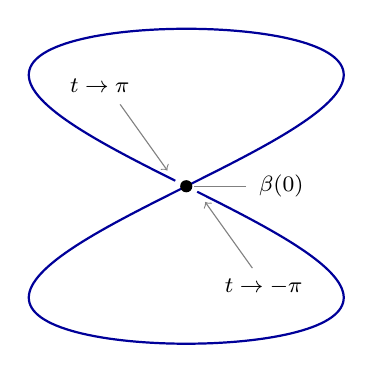
\begin{tikzpicture}[scale=2.0]
\draw[blue!60!black,thick,domain=-178:178,samples=250,variable=\t] plot ({sin(2*\t)},{sin(\t)});
\fill (0,0) circle (1.1pt);
\node[font=\footnotesize,anchor=west] at (0.40,0) {$\beta(0)$};
\draw[gray] (0.38,0)--(0.05,0);
\node[font=\footnotesize,anchor=west] at (-0.80,0.64) {$t\to\pi$};
\node[font=\footnotesize,anchor=east] at (0.80,-0.64) {$t\to-\pi$};
\draw[->,gray] (-0.42,0.52)--(-0.12,0.10);
\draw[->,gray] (0.42,-0.52)--(0.12,-0.10);
\end{tikzpicture}
\caption{例~\ref{A:ex:fig8}：$\beta(t)=(\sin2t,\sin t)$、$t\in(-\pi,\pi)$。像は 8 の字だが、$t\to\pm\pi$ の端が $t=0$ の点に近づくので、像の位相は区間 $(-\pi,\pi)$ の位相と異なる。}\label{A:fig:fig8}
\end{figure}

\begin{ex}[トーラス上の無理数傾きの直線]\label{A:ex:irr}
$a$ を無理数として $\gamma:\R\to T^2=\R^2/\Z^2$、$\gamma(t)=[(t,at)]$。微分は $(1,a)\ne0$、単射（$t\ne s$ で $(t-s,a(t-s))\in\Z^2$ なら $t-s=k\in\Z\setminus0$ かつ $ak\in\Z$ で矛盾）。像は $T^2$ で稠密（Kronecker：$\{na\bmod1\}$ が稠密）である。もし埋め込みなら像は 1 次元の埋め込み部分多様体で、スライス座標により\emph{局所閉集合}（開集合と閉集合の共通部分）である。稠密な局所閉集合 $O\cap C$ は $C=T^2$ となるので開集合だが、$T^2$ の空でない開集合は 1 次元部分多様体になれない（スライス座標が $\varphi(U\cap S)\subset\R\times0$ で、$\varphi(U)$ が開なので不可能）。ゆえに埋め込みでない（問~\ref{pr:A_irrational}）。
\end{ex}

\begin{thm}[Whitney の埋め込み定理]
$n$ 次元の（第2可算 Hausdorff）多様体は $\R^{2n}$ に埋め込める。
\end{thm}
\tC\ Lee 第 6 章。弱い版（$\R^{2n+1}$）は 1 の分割と Sard の定理から比較的容易に示せる。「多様体 = $\R^N$ の部分多様体」と思ってよいので、具体例では $\R^N$ の部分多様体として扱うことが多い。

\subsection{1 の分割}
\paragraph{動機。}多様体上の構造（計量、接続、積分など）は、局所座標では簡単に作れても、大域的に作るには局所構造を貼り合わせる必要がある。局所構造が「凸結合」できるものなら、\emph{1 の分割}で貼り合わせられる。以後の巻の存在定理（Riemann 計量、Hermite 計量、接続の存在、積分の定義）はほぼすべてこの手法による。

\begin{lem}[バンプ関数]\label{A:lem:bump}
\tP\ $h(t)=e^{-1/t}$（$t>0$）、$h(t)=0$（$t\le0$）は $C^\infty$。$\R^n$ の点 $a$ と $r>0$ に対し、$\bar B_{r/2}(a)$ 上で $1$、$B_r(a)$ の外で $0$、$0\le b\le1$ で、$\operatorname{supp}b\subset\bar B_r(a)$ の滑らかな関数 $b:\R^n\to\R$ がある。
\end{lem}
\begin{proof}
$t>0$ で $h^{(k)}(t)=P_k(1/t)e^{-1/t}$（$P_k$ は多項式）が帰納的に成り立ち、$t\to0^+$ で $s=1/t\to\infty$ より $P_k(s)e^{-s}\to0$。よって $h^{(k)}(0)=0$ で $h\in C^\infty(\R)$。$\lambda(t)=\dfrac{h(t)}{h(t)+h(1-t)}$ は $t\le0$ で $0$、$t\ge1$ で $1$ の滑らかな関数（分母は零にならない）。$b(x)=1-\lambda\bigl(\frac{2|x-a|}{r}-1\bigr)$ とおく：$|x-a|\le r/2$ で $\frac{2|x-a|}r-1\le0$ より $\lambda=0$、$b=1$、$|x-a|\ge r$ で $\lambda=1$ より $b=0$。$|x-a|$ は $x\ne a$ で滑らかで、$x=a$ の近傍（$|x-a|<r/2$）では $b\equiv1$ だから、$b$ は $\R^n$ 全体で滑らか。
\end{proof}

\begin{defn}[1 の分割]
$M$ の開被覆 $\{U_\alpha\}_{\alpha\in A}$ に\emph{従属する 1 の分割}（partition of unity）とは、滑らかな関数 $\rho_\alpha:M\to[0,1]$ の族で、(i) $\operatorname{supp}\rho_\alpha\subset U_\alpha$、(ii) \emph{局所有限}（各点に、$\operatorname{supp}\rho_\alpha$ のうち有限個としか交わらない近傍がある）、(iii) $\sum_\alpha\rho_\alpha\equiv1$ を満たすもの。
\end{defn}

\begin{figure}[htbp]
\centering
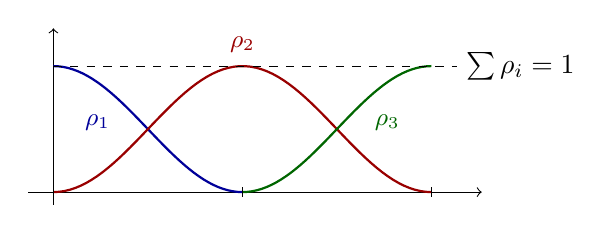
\begin{tikzpicture}[scale=1.6]
\draw[->] (-0.2,0)--(3.4,0); \draw[->] (0,-0.1)--(0,1.3);
\draw[blue!60!black,thick,domain=0:1.5,samples=40] plot (\x,{(cos(60*\x))^2});
\draw[red!60!black,thick,domain=0:3,samples=70] plot (\x,{(cos(60*(\x-1.5)))^2});
\draw[green!40!black,thick,domain=1.5:3,samples=40] plot (\x,{(cos(60*(\x-3)))^2});
\draw[dashed] (0,1)--(3.2,1) node[right]{$\sum\rho_i=1$};
\node[blue!60!black,font=\small] at (0.35,0.55) {$\rho_1$};
\node[red!60!black,font=\small] at (1.5,1.17) {$\rho_2$};
\node[green!40!black,font=\small] at (2.65,0.55) {$\rho_3$};
\foreach \x/\n in {0/0,1.5/1.5,3/3} {\draw (\x,0.04)--(\x,-0.04);}
\end{tikzpicture}
\caption{1 の分割の模式図（区間 $[0,3]$、$\rho_i$ は $\cos^2$ の山を使った $C^1$ 級の模型。本物は $h(t)=e^{-1/t}$ を使って $C^\infty$ にする）。各点で、重なる 2 つの関数の和が $1$ になる。}
\end{figure}

\begin{thm}[1 の分割の存在]\label{A:thm:pou}
\tP\ $M$ を（Hausdorff、第2可算な）滑らかな多様体、$\{U_\alpha\}$ を開被覆とする。このとき $\{U_\alpha\}$ に従属する 1 の分割で、さらに各 $\rho_\alpha$ のサポートがコンパクトであるような可算族 $\{\rho_k\}_{k\ge1}$（$\operatorname{supp}\rho_k\subset U_{\alpha(k)}$）が存在する。
\end{thm}
\begin{proof}
\emph{Step 1（コンパクト列による尽くし）。}$M$ は局所コンパクト（座標球の閉包はコンパクト）で、閉包がコンパクトな座標球たちは基底をなす。第2可算性から、そのうち可算個で基底になるもの $B_1,B_2,\dots$ がとれる（可算基底 $\{C_i\}$ をとり、$C_i\subset B\subset C_j$ となる座標球 $B$ が存在する各組 $(i,j)$ に対し 1 つずつ $B_{ij}$ を選べば、$\{B_{ij}\}$ が基底になる）。$K_1=\bar B_1$、帰納的に $m_j\ge j+1$ を $K_j\subset B_1\cup\dots\cup B_{m_j}$ となる最小の整数としてとり、$K_{j+1}=\bar B_1\cup\dots\cup\bar B_{m_j}$ とおく。各 $K_j$ はコンパクトで $K_j\subset\operatorname{int}K_{j+1}$、$\bigcup K_j=M$（$B_j\subset K_{j+1}$）。$K_0=K_{-1}=\emptyset$ とする。

\emph{Step 2（局所的な山を作る）。}$A_j=K_j\setminus\operatorname{int}K_{j-1}$（コンパクト）、$W_j=\operatorname{int}K_{j+1}\setminus K_{j-2}$（開。$K_{j-2}$ はコンパクトなので Hausdorff 性より閉）とおくと $A_j\subset W_j$（$K_{j-2}\subset\operatorname{int}K_{j-1}$ より）、$\bigcup_jA_j=M$。各 $p\in A_j$ に対し、$p\in U_\alpha$ となる $\alpha$ をとり、座標近傍 $(U',\varphi)$ で $p\in U'\subset U_\alpha\cap W_j$、$\varphi(p)=0$、$\varphi(U')\supset\bar B_{2r}(0)$ となるものを選ぶ。補題~\ref{A:lem:bump} の $b$（$a=0$、半径 $r$）を用いて $b_p=b\circ\varphi$（$\varphi^{-1}(\bar B_{2r})$ の中）、それ以外で $0$ とおく。$\varphi^{-1}(\bar B_r)$ はコンパクト、したがって（Hausdorff より）閉なので、$b_p$ は $M$ 上で滑らかで、$b_p(p)=1$、$\operatorname{supp}b_p\subset\varphi^{-1}(\bar B_r)\subset U_\alpha\cap W_j$ をみたす。$\{b_p>0\}$ は $p$ の開近傍で、$A_j$ のコンパクト性により有限個の $p_{j,1},\dots,p_{j,r_j}\in A_j$ で $A_j\subset\bigcup_s\{b_{p_{j,s}}>0\}$ となる。

\emph{Step 3（局所有限性と正規化）。}族 $\{b_{p_{j,s}}\}_{j,s}$ は可算である。局所有限：任意の点 $q$ は $\operatorname{int}K_N$ のある $N$ に入り、$j\ge N+2$ なら $\operatorname{supp}b_{p_{j,s}}\subset W_j\subset M\setminus K_{j-2}\subset M\setminus K_N$ なので $\operatorname{int}K_N$ と交わらない。したがって $\operatorname{int}K_N$ と交わるのは $j\le N+1$ の有限個のみ。和 $\Psi=\sum_{j,s}b_{p_{j,s}}$ は各点の近傍で有限和ゆえ滑らかで、$\bigcup A_j=M$ と Step 2 から $\Psi>0$。$\rho_{(j,s)}=b_{p_{j,s}}/\Psi$ が求める 1 の分割。各 $\operatorname{supp}\rho$ はコンパクトで、ある $U_\alpha$ に含まれる。
\end{proof}
\begin{rem}[添字のまとめ方]
定理の $\{\rho_k\}$ の添字は可算集合 $\{k\}$ で、$\alpha(k)$ は各 $k$ に対して選んだ $\alpha$ である。そこで $\rho_\alpha:=\sum_{k:\,\alpha(k)=\alpha}\rho_k$（該当する $k$ がなければ $0$）とおくと、局所有限性より各点の近傍で有限和なので $\rho_\alpha$ は滑らかで、$\operatorname{supp}\rho_\alpha\subset U_\alpha$ かつ $\sum_\alpha\rho_\alpha\equiv1$ である（局所有限な族では、台の和集合の閉包は台の閉包の和集合になる）。こうして、定義どおり開被覆と同じ添字集合 $A$ で番号づけられた 1 の分割が得られる（台のコンパクト性は失ってよい）。以下で「従属する 1 の分割 $\{\rho_\alpha\}$」というときは、この形のものを使う。
\end{rem}

\begin{cor}\label{A:cor:pou}
\tP\ (a) $A\subset U\subset M$、$A$ 閉、$U$ 開のとき、$A$ 上 $1$、$\operatorname{supp}f\subset U$ の滑らかな関数 $f:M\to[0,1]$ がある。(b) 局所定義された滑らかな構造の貼り合わせ：座標近傍ごとに作った「正値な対称 2 階テンソル（計量）」「正値な内積」などは、1 の分割で凸結合すれば大域的な対象になる（§6、§7）。(c) 滑らかな\emph{固有関数} $f:M\to[0,\infty)$（$f^{-1}([0,c])$ がコンパクト）が存在する（問~\ref{pr:A_proper}）。
\end{cor}
\begin{proof}
(a) 被覆 $\{U,M\setminus A\}$ に従属する 1 の分割 $\{\rho_U,\rho_{M\setminus A}\}$ をとり $f=\rho_U$：$A$ 上 $\rho_{M\setminus A}=0$ より $\rho_U=1$。
\end{proof}

\subsection{境界つき多様体}
閉区間 $[0,1]$、閉円盤 $D^n$、円柱 $S^1\times[0,1]$ は座標近傍が $\R^n$ の開集合でなく、半空間 $\mathbb H^n=\{x\in\R^n:x^n\ge0\}$ の開集合（相対位相）と同相になる点をもつ。

\begin{defn}
\emph{境界つき $n$ 次元多様体} $M$ は、Hausdorff、第2可算で、各点が $\R^n$ または $\mathbb H^n$ の開集合と同相な近傍をもつもの。座標変換が滑らかである（半空間の開集合上の写像が滑らかとは、局所的に $\R^n$ の開集合上の滑らかな写像に延びること）とき滑らかという。$x^n=0$ に写される点の全体を \emph{境界} $\partial M$、残りを\emph{内部} $\operatorname{int}M$ という。
\end{defn}
内部の点と境界の点は座標のとり方によらず区別でき（逆関数定理から従う\tC）、$\partial M$ は $(n-1)$ 次元の（境界のない）多様体、$\operatorname{int}M$ は $n$ 次元の多様体になる。$\partial M$ がコンパクト・空でもよい（例：$[0,1]$ は $\partial=\{0,1\}$、$D^n$ は $\partial=S^{n-1}$）。

\begin{figure}[htbp]
\centering
\begin{tikzpicture}[>={Stealth[length=2.2mm]},scale=1.0]
\draw[thick,fill=gray!8] (0,0) circle (1.4);
\draw[blue!60!black,thick,fill=blue!15] (1.4,0) arc (0:45:1.4) -- ++(-0.55,-0.1) arc (60:-60:0.9)-- cycle;
\fill[blue!25,opacity=0.7] (0.95,0.95) ellipse (0.45 and 0.35);
\node at (-0.2,-0.3) {$D^2$};
\node at (0.4,1.7) {\small $\partial D^2=S^1$};
\draw[->,thick] (2.0,0.2)--(3.3,0.2) node[midway,above]{$\varphi$};
\fill[gray!10] (3.5,-1.2) rectangle (7,1.5);
\draw[thick] (3.5,-0.4)--(7,-0.4);
\fill[blue!25] (4.7,-0.4) arc (180:0:0.8) -- cycle;
\draw[blue!60!black,thick] (4.7,-0.4) arc (180:0:0.8);
\node[font=\small] at (6.2,1.1) {$\mathbb H^2=\{x^2\ge0\}$};
\node[font=\small] at (6.2,-0.75) {$\{x^2=0\}$};
\end{tikzpicture}
\caption{境界つき多様体の座標。円盤の境界付近の座標近傍は、半空間 $\mathbb H^2$ の開集合（半円盤）と同一視される。}
\end{figure}

\begin{prop}\label{A:prop:halfspace}
$f:M\to\R$ が滑らかで $0$ が $f$ の正則値のとき、$\{f\ge0\}$ は（$M$ の中の）境界つき $n$ 次元多様体で、境界は $\{f=0\}$ である（証明は問~\ref{pr:A_disc}）。たとえば $f=1-|x|^2$ で $D^n$。
\end{prop}

境界つき多様体の積には角ができる（$[0,1]^2$）ので、丸めて考えるか、角つき多様体を使う。本巻では角は扱わない。

\subsection{向き}\label{A:sub:orient}
\paragraph{動機。}積分（§4）で $\int_M\omega$ を定義するには、座標を取り替えたとき Jacobi 行列式の符号が変わらないように座標を選んでおく必要がある。これが「向き」である。線形代数的には、$V$ の基底の向き（$\det P>0$ で同じ向き）の選択に対応する。

\begin{defn}
アトラス $\{(U_\alpha,\varphi_\alpha)\}$ が\emph{向きづけられている}とは、すべての座標変換の Jacobi 行列式が正であること。\emph{向きづけ可能}（orientable）とは、向きづけられたアトラスをもつこと。向きづけられた極大アトラスを選ぶことを\emph{向き}を与えるという。座標近傍が向きと整合するとき正の向きの座標近傍という。
\end{defn}

\begin{lem}\label{A:lem:orient2}
\tP\ 連結な向きづけ可能多様体の向きは、ちょうど 2 つある（互いに逆）。
\end{lem}
\begin{proof}
向き $\mathcal O$ を固定する。別の向き $\mathcal O'$ に対し、$p\in M$ で $\mathcal O'$ の座標近傍の（$\mathcal O$ の座標近傍に対する）Jacobi 行列式の符号 $s(p)\in\{\pm1\}$ は、座標近傍の選び方によらず（座標変換の行列式は $\mathcal O$ の中で正、$\mathcal O'$ の中で正）、局所定数。連結だから $s$ は定数 $\pm1$。$s=1$ なら $\mathcal O'=\mathcal O$、$s=-1$ なら $\mathcal O'=-\mathcal O$（1 つ目の座標を反転）。
\end{proof}

\begin{ex}
(1) $\R^n$、およびその開集合は向きづけ可能。(2) 積 $M\times N$ は、両方が向きづけ可能なら向きづけ可能。特に $T^n$ は向きづけ可能（実際 $T^n$ には $\dd\theta^1\wedge\dots\wedge\dd\theta^n$ が至るところ $\ne0$）。(3) $S^n$ は向きづけ可能：立体射影 2 枚の座標変換 $u\mapsto u/|u|^2$ の Jacobi 行列式は $-|u|^{-2n}<0$（問~\ref{pr:A_stereo}）なので、$\sigma_S$ の第 1 座標の符号を反転した座標 $r\circ\sigma_S$ を使えば、行列式が正になって向きづけられたアトラスができる。
\end{ex}

\paragraph{向きづけ不可能な例：被覆の議論。}$p:\tilde M\to M$ を局所微分同相、$T:\tilde M\to\tilde M$ を $p\circ T=p$ を満たす微分同相（被覆変換）とする。

\begin{lem}\label{A:lem:covorient}
\tP\ $\tilde M$ が連結で、向き $\mathcal O$ と点 $x\in\tilde M$ について、$x$ の近傍の $\mathcal O$ の座標近傍 $\chi$ と $T(x)$ の近傍の $\mathcal O$ の座標近傍 $\chi'$ に対し $\chi'\circ T\circ\chi^{-1}$ の Jacobi 行列式が $\chi(x)$ で負である（$T$ は $\mathcal O$ の向きを\emph{逆転する}）ならば、$M$ は向きづけ不可能である。
\end{lem}
\begin{proof}
$M$ に向きづけられたアトラス $\{(V_a,\psi_a)\}$ があったとする。$p$ が単射となる開集合 $W\subset\tilde M$ に対して $\chi=\psi_a\circ p|_W$（$p(W)\subset V_a$）は $\tilde M$ の座標近傍で、これらは向きづけられたアトラスをなす（座標変換は $\psi_b\psi_a^{-1}$ の制限）。それを $\mathcal O_p$ とする。$\tilde M$ は連結だから補題~\ref{A:lem:orient2} より $\mathcal O_p=\pm\mathcal O$。$T$ が $\mathcal O$ の向きを逆転するなら $-\mathcal O$ の向きも逆転する（$\chi,\chi'$ の両方に反転を合成しても $\chi'T\chi^{-1}$ の Jacobi 行列式の符号は変わらない）ので、$T$ は $\mathcal O_p$ を逆転する。一方、$x\in W$ として $\chi=\psi_a\circ p|_W$ と $\chi'=\psi_a\circ p|_{T(W)}$（$p\circ T=p$ より $p|_{T(W)}$ も単射で $p(T(W))=p(W)\subset V_a$）について $\chi'\circ T=\psi_a\circ p\circ T|_W=\psi_a\circ p|_W=\chi$、すなわち $\chi'\circ T\circ\chi^{-1}=\mathrm{id}$ で Jacobi 行列式は $1>0$。矛盾。
\end{proof}

\begin{ex}[Möbius の帯]\label{A:ex:mobius}
$\tilde M=\R\times(-1,1)$（連結）、$T(x,y)=(x+1,-y)$。$\langle T\rangle\cong\Z$ は $\tilde M$ に自由かつ固有不連続に作用し、商 $M=\tilde M/\langle T\rangle$（\emph{Möbius の帯}）は 2 次元多様体で、射影は局所微分同相である\tC（Lee 第 21 章）。$T$ の Jacobi 行列は $\operatorname{diag}(1,-1)$ で行列式 $-1<0$（標準座標は向き $\mathcal O$ を与え、$T$ が逆転する）。補題~\ref{A:lem:covorient} より Möbius の帯は向きづけ不可能。
\end{ex}

\begin{ex}[$\RP^2$]\label{A:ex:RP2}
$p:S^2\to\RP^2$ は局所微分同相（半球面 $\{x_i>0\}$ から $\R^2$ への $x\mapsto(x_j/x_i)_{j\ne i}$ が同型）で、対蹠写像 $T(x)=-x$ が被覆変換。立体射影 $\sigma_N$ による座標で $T$ は、$S^2\setminus\{N,S\}$ 上で $\sigma_N T\sigma_N^{-1}(u)=-u/|u|^2$（$x\mapsto-x$ のとき $u=\frac{x'}{1-x_3}\mapsto\frac{-x'}{1+x_3}$ で、$|u|^2=\frac{1+x_3}{1-x_3}$ より $-u/|u|^2$）。反転 $u\mapsto u/|u|^2$ の Jacobi 行列式は $-|u|^{-2n}$（$n=2$）、$u\mapsto-u$ のそれは $(-1)^n=1$。合成の行列式は $-|u|^{-4}<0$。$S^2\setminus\{N\}\cong\R^2$ は連結で $\sigma_N$ は（符号が一定の）向きの座標だから、$T$ は向きを逆転する。ゆえに $\RP^2$ は向きづけ不可能（補題~\ref{A:lem:covorient}）。同じ計算で、一般の偶数 $n$ について $\RP^n$ は向きづけ不可能、奇数 $n$ なら向きづけ可能（$\RP^1=S^1$、$\RP^3=\SO(3)$）。
\end{ex}

\begin{figure}[htbp]
\centering
\begin{tikzpicture}[>={Stealth[length=2.2mm]},scale=1.0]
\def\dbl{-{Latex[length=2mm]Latex[length=2mm]}}
% Moebius
\draw[thick,fill=blue!6] (0,0) rectangle (4,2);
\draw[->,very thick,red!70!black] (0,0.2)--(0,1.2);
\draw[->,very thick,red!70!black] (4,1.8)--(4,0.8);
\node at (2,1) {Möbius の帯};
\draw[->,thick,gray] (0.7,0.5)--(1.3,0.5);
\draw[->,thick,gray] (0.7,0.5)--(0.7,1.1);
\draw[->,thick,gray] (3.3,1.5)--(2.7,1.5);
\draw[->,thick,gray] (3.3,1.5)--(3.3,0.9);
\node[font=\footnotesize] at (2,-0.4) {$(x,y)\sim(x+1,-y)$};
% torus
\draw[thick,fill=blue!6] (6,0) rectangle (9,2);
\draw[->,very thick,red!70!black] (6,0.5)--(6,1.5);
\draw[->,very thick,red!70!black] (9,0.5)--(9,1.5);
\draw[very thick,blue!60!black,\dbl] (6.7,0)--(8.4,0);
\draw[very thick,blue!60!black,\dbl] (6.7,2)--(8.4,2);
\node at (7.5,1) {トーラス $T^2$};
\node[font=\footnotesize] at (7.5,-0.4) {辺を同じ向きに貼る};
\end{tikzpicture}
\caption{左：Möbius の帯は長方形の左右の辺を（上下を反転して）貼り合わせたもの。図の灰色の座標軸の組（枠）を右の辺まで運ぶと、帯を一周して戻ったとき向きが逆になる。右：トーラスは向きがそのまま貼り合うので向きづけ可能。}\label{A:fig:mobius}
\end{figure}

\subsection{曲面の分類（言及）}
\begin{thm}[コンパクト曲面の分類]\label{A:thm:surfaces}
\tC\ 連結でコンパクトな境界のない曲面は、次のいずれかと微分同相である。(i) 向きづけ可能：種数 $g\ge0$ の曲面 $\Sigma_g=T^2\#\cdots\#T^2$（$g=0$ は $S^2$）、Euler 標数 $\chi=2-2g$。(ii) 向きづけ不可能：$k\ge1$ 個の $\RP^2$ の連結和 $\#_k\RP^2$、$\chi=2-k$。
\end{thm}
\src{Lee『Introduction to Topological Manifolds』第 6 章、Hatcher『Algebraic Topology』第 1 章 §1.2\tQ。多様体としての微分同相は、位相同相から従う（2 次元の特殊事情）。}

\begin{figure}[htbp]
\centering
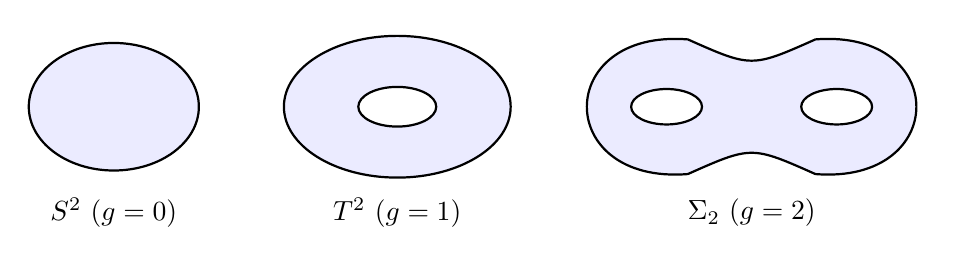
\begin{tikzpicture}[scale=0.9]
\draw[thick,fill=blue!8] (0,0) ellipse (1.2 and 0.9);
\node at (0,-1.5) {$S^2$ ($g=0$)};
\begin{scope}[xshift=4.0cm]
\draw[thick,fill=blue!8] (0,0) ellipse (1.6 and 1.0);
\draw[thick,fill=white] (0,0) ellipse (0.55 and 0.28);
\node at (0,-1.5) {$T^2$ ($g=1$)};
\end{scope}
\begin{scope}[xshift=9.0cm]
\draw[thick,fill=blue!8] (-0.9,0.95) .. controls (0,0.55) .. (0.9,0.95) .. controls (2.8,1.1) and (2.8,-1.1) .. (0.9,-0.95) .. controls (0,-0.55) .. (-0.9,-0.95) .. controls (-2.8,-1.1) and (-2.8,1.1) .. (-0.9,0.95)--cycle;
\draw[thick,fill=white] (-1.2,0) ellipse (0.5 and 0.25);
\draw[thick,fill=white] (1.2,0) ellipse (0.5 and 0.25);
\node at (0,-1.5) {$\Sigma_2$ ($g=2$)};
\end{scope}
\end{tikzpicture}
\caption{向きづけ可能なコンパクト曲面。穴の個数が種数 $g$。}
\end{figure}

3 次元では、境界のないコンパクトな単連結 3 次元多様体がすべて $S^3$ と微分同相であること（Poincaré 予想、Perelman）、4 次元以上では分類が（アルゴリズム的に）不可能であることが知られている\tC。

\begin{keybox}{§2 の要点}
\begin{itemize}
\item 多様体 $=$ Hausdorff・第2可算な位相空間 $+$ 滑らかに貼り合うアトラス（座標近傍の族）。座標変換が滑らかであることが本質。
\item 例：$\R^n$、開集合、$S^n$（立体射影 2 枚、変換 $u\mapsto u/|u|^2$）、$T^n$、$\RP^n$、$\CP^n$、$\GL(n,\R)$、$\SO(n)$（$\dim=\frac{n(n-1)}{2}$）。
\item \textbf{正則値定理}：$c$ が正則値なら $F^{-1}(c)$ は余次元 $n$ の部分多様体。局所標準形（沈め込み $\to$ 射影、はめ込み $\to$ 包含）は逆関数定理の帰結。
\item 埋め込み $=$ はめ込み $+$ 像への同相。単射なはめ込みでも埋め込みとは限らない（8 の字、無理数傾きの線）。コンパクト／固有なら大丈夫。
\item \textbf{1 の分割}は局所構造を貼り合わせる標準手段。存在の証明には Hausdorff と第2可算が効く。
\item 向きづけ可能 $\Leftrightarrow$ 座標変換の Jacobi 行列式が正のアトラスがある。Möbius の帯、$\RP^{2m}$ は向きづけ不可能。
\end{itemize}
\end{keybox}

\subsection*{§2 のつまずきやすい点}
\begin{enumerate}
\item \textbf{位相多様体の条件の Hausdorff・第2可算を忘れる。}局所 Euclid だけでは病的な例（原点が 2 つの直線）が出る。
\item \textbf{滑らかな構造は「アトラスの同値類」。}同じ集合に異なる滑らかな構造を入れうる。微分同相という弱い同値関係で見ると、これらが同じになる場合も多い。
\item \textbf{$\operatorname{rank}$ は座標によらないが、$\det$ や符号はよる。}向きは Jacobi 行列式の\emph{符号}に関する情報で、座標の取り方に依存する。
\item \textbf{正則値の定義：$F^{-1}(c)$ のすべての点で $dF$ が全射。}1 点でも臨界点があると $F^{-1}(c)$ は多様体とは限らない（$F=xy$、$c=0$ は十字形）。
\item \textbf{部分多様体と部分集合の位相。}はめ込まれた多様体は、像に部分空間位相を入れた多様体とは限らない（8 の字）。
\end{enumerate}

\subsection*{§2 の問題}

\begin{probl}{基本}{A_stereo}
$S^n$ の立体射影について (a) $\sigma_N^{-1}$ が例~\ref{A:ex:Sn} の式で与えられることを確かめよ。(b) 反転 $\iota(u)=u/|u|^2$ の Jacobi 行列は $\frac1{|u|^2}\bigl(I-2\hat u\hat u^T\bigr)$（$\hat u=u/|u|$）で、行列式は $-|u|^{-2n}$ であることを示せ。(c) $r(v_1,\dots,v_n)=(-v_1,v_2,\dots,v_n)$ とおくと、$\{\sigma_N,\ r\circ\sigma_S\}$ は向きづけられたアトラスをなす（$S^n$ の向きづけ可能性）ことを示せ。
\end{probl}

\begin{probl}{標準}{A_cp1}
$\CP^1$ の 2 枚の座標 $z=z_1/z_0$、$w=z_0/z_1$（$w=1/z$）と、$S^2$ の座標 $\sigma_N$、$\overline{\ \cdot\ }\circ\sigma_S$（$\sigma_S$ に複素共役 $r'(v_1,v_2)=(v_1,-v_2)$ を合成したものを $\C$ の座標とみなす）を考える。$S^2\to\CP^1$ を、$S^2\setminus\{N\}$ では $x\mapsto[1:\sigma_N(x)]$（$\sigma_N(x)\in\R^2=\C$）、$N\mapsto[0:1]$ で定める。これが微分同相であることを示せ。\hint{$\sigma_S(x)=\sigma_N(x)/|\sigma_N(x)|^2$ を複素数で書くと $\overline{\sigma_S}=1/\sigma_N$}
\end{probl}

\begin{probl}{標準}{A_rp}
(a) $\RP^2$ の座標 $\varphi_0[x]=(x_1/x_0,x_2/x_0)=(y_1,y_2)$ と $\varphi_1[x]=(x_0/x_1,x_2/x_1)=(u,v)$ について、座標変換 $\varphi_0\circ\varphi_1^{-1}$ を求め、その Jacobi 行列式が $-1/u^3$ であることを示せ。(b) $\RP^1\to S^1$、$[x_0:x_1]\mapsto\bigl(\frac{x_0^2-x_1^2}{x_0^2+x_1^2},\frac{2x_0x_1}{x_0^2+x_1^2}\bigr)$ が微分同相であることを示せ。\hint{(b) $[\cos\theta:\sin\theta]\mapsto(\cos2\theta,\sin2\theta)$。像から $(-1,0)$ を除いた座標で見る}
\end{probl}

\begin{probl}{標準}{A_sl}
(a) $\SL(n,\R)$ が $n^2-1$ 次元の多様体であることを示せ（$D\det_A(H)=\det A\,\tr(A^{-1}H)$ を使う。この公式は $\det(A+tH)=\det A\det(I+tA^{-1}H)$ から得よ）。(b) $\SO(3)$ が 3 次元であることを例~\ref{A:ex:SOn} の方法で確かめ、$\SO(3)$ の単位元での「接空間」$\ker DF_I$ が歪対称行列の空間であること、その次元が 3 であることを確かめよ。(c) $\U(n)$ が $n^2$ 次元の多様体であることを示せ（(b) と同様に $F(A)=A^*A$ を考える）。
\end{probl}

\begin{probl}{標準}{A_torus}
$F(x,y,z)=\bigl(\sqrt{x^2+y^2}-2\bigr)^2+z^2$ とする（$\R^3\setminus\{(0,0,z)\}$ 上で滑らか）。(a) $1$ が正則値であることを示し、$F^{-1}(1)$ がコンパクトな 2 次元部分多様体（トーラス）であることを示せ。(b) 写像 $T^2\to F^{-1}(1)$、$(\theta,\phi)\mapsto\bigl((2+\cos\phi)\cos\theta,(2+\cos\phi)\sin\theta,\sin\phi\bigr)$ が微分同相であることを、はめ込み・単射・コンパクトを使って示せ。
\end{probl}

\begin{probl}{標準}{A_fig8}
例~\ref{A:ex:fig8} の $\beta$ が (a) はめ込みで、(b) 単射であることを示し、(c) $\beta$ が埋め込みでないことを示せ。\hint{(b) $\sin t=\sin s$ なら $s=t$ か $s=\pi-t$。(c) $\beta$ が像への同相なら $t=0$ の小さな開区間の像は像の中で開。}
\end{probl}

\begin{probl}{標準}{A_irrational}
例~\ref{A:ex:irr} について (a) $\{na\bmod1:n\in\Z\}$ が $S^1=\R/\Z$ で稠密であることを（鳩の巣原理で）示せ。(b) 従って像 $\gamma(\R)$ が $T^2$ で稠密であることを示せ。(c) $\gamma$ が埋め込みでないことを示せ。
\end{probl}

\begin{probl}{基本}{A_bump}
(a) $h(t)=e^{-1/t}$（$t>0$）、$0$（$t\le0$）が $t=0$ で $C^\infty$ であることを示せ。(b) $S^1$（角度 $\theta\in\R/2\pi\Z$）の開被覆 $U_1=S^1\setminus\{\theta=0\}$、$U_2=S^1\setminus\{\theta=\pi\}$ に従属する 1 の分割を具体的に作れ。
\end{probl}

\begin{probl}{発展}{A_proper}
$M$ に滑らかな関数 $f:M\to[0,\infty)$ で、固有（$\{f\le c\}$ がコンパクト）となるものがあることを示せ。\hint{定理~\ref{A:thm:pou} の 1 の分割 $\{\rho_k\}$（サポートがコンパクト）に対し $f=\sum_kk\rho_k$。}
\end{probl}

\begin{probl}{標準}{A_disc}
$f:M\to\R$ が滑らかで $0$ が正則値とする。$N=\{f\ge0\}$ が境界つき多様体で $\partial N=\{f=0\}$ であることを示せ。\hint{$f(p)=0$ の点で、座標を $(y^1,\dots,y^{n-1},f)$ にとる。}
\end{probl}

\begin{probl}{標準}{A_klein}
$a(x,y)=(x+1,-y)$、$b(x,y)=(x,y+1)$ が生成する $\R^2$ 上の変換群 $\Gamma$ をとる（$aba^{-1}=b^{-1}$）。商 $K=\R^2/\Gamma$（\emph{Klein の壺}）は、補題~\ref{A:lem:covorient} により向きづけ不可能であることを示せ。また $\R^2/\langle(x,y)\mapsto(x+1,y),(x,y)\mapsto(x,y+1)\rangle=T^2$ が向きづけ可能であることも確かめよ。
\end{probl}

%==================================================
\section{接空間・ベクトル場・Lie 括弧・Frobenius の定理}\label{A:sec3}
%==================================================
\begin{goalbox}{この節の位置づけ}
多様体の各点での「速度」＝接ベクトルを 3 通りに定義し、それらが同値であることを示す。微分 $\dd F$、接束 $TM$、ベクトル場、その流れ（ODE）、そして 2 つのベクトル場から 1 つを作る\textbf{Lie 括弧}を学ぶ。Lie 括弧は流れの非可換性を測る量であり、Lie 群の Lie 代数、分布の可積分性（\textbf{Frobenius の定理}）、そして §4 以降の外微分と Cartan の公式の核になる。
\end{goalbox}

\subsection{接ベクトル：3 つの定義}
\paragraph{動機。}$\R^n$ の点 $p$ での接ベクトルは、単に $\R^n$ のベクトルである。$\R^n$ のベクトル $v$ は、(i) 関数 $f$ の $v$ 方向の方向微分 $\partial_vf(p)=\sum v^i\partial_if(p)$ を与え、(ii) 曲線 $t\mapsto p+tv$ の速度であり、(iii) 成分 $(v^1,\dots,v^n)$ をもつ。多様体には周囲のベクトル空間がないので、これら 3 つの側面のどれか（またはすべて）を使って「内在的に」定義する。そして 3 つが一致することを確かめる。

$M$ を $n$ 次元の滑らかな多様体、$p\in M$ とする。

\begin{defn}[接ベクトルの 3 つの定義]\label{A:def:tangent}
\begin{enumerate}
\item[(A)]（導分）\ $v:C^\infty(M)\to\R$ が線形で Leibniz 則 $v(fg)=f(p)\,v(g)+g(p)\,v(f)$ を満たすとき、$v$ を $p$ での\emph{接ベクトル}（導分、derivation）という。その全体を $T_pM$ と書く。
\item[(B)]（曲線の速度）\ $\gamma:(-\varepsilon,\varepsilon)\to M$、$\gamma(0)=p$ の滑らかな曲線 $\gamma,\gamma'$ が同値とは、$p$ のある（従ってすべての）座標近傍 $(U,\varphi)$ で $(\varphi\circ\gamma)'(0)=(\varphi\circ\gamma')'(0)$ が成り立つこと。同値類 $[\gamma]$ を接ベクトルという。
\item[(C)]（成分）\ 各座標近傍 $(U,x)$ ごとに $v^i\in\R$（$i=1,\dots,n$）を与え、座標を $y=y(x)$ に取り替えたとき
\[
v'^j=\frac{\partial y^j}{\partial x^i}(p)\,v^i
\]
で変換するもの。
\end{enumerate}
\end{defn}

(B) の同値性が座標によらないのは連鎖律による：$\psi\circ\gamma=(\psi\circ\varphi^{-1})\circ(\varphi\circ\gamma)$ だから $(\psi\circ\gamma)'(0)=D(\psi\varphi^{-1})\,(\varphi\gamma)'(0)$。これは (C) の変換則そのものである。

\begin{lem}[局所性と Hadamard の補題]\label{A:lem:hadamard}
\tP\ (a) $v\in T_pM$ で、$f\in C^\infty(M)$ が $p$ の近傍で $0$ ならば $v(f)=0$。特に $v(f)$ は $f$ の $p$ のまわりでの値のみに依る（$p$ の近傍でのみ定義された関数にも $v$ は作用する）。(b) $v(c)=0$（定数関数 $c$）。(c) $B\subset\R^n$ が原点を中心とする球、$f\in C^\infty(B)$ なら $f(x)=f(0)+\sum_ix^ig_i(x)$、$g_i\in C^\infty(B)$、$g_i(0)=\partial_if(0)$。
\end{lem}
\begin{proof}
(a) $f=0$ が $W\ni p$ で成り立つとする。補題~\ref{A:lem:bump} と系~\ref{A:cor:pou}(a) により $\chi\in C^\infty(M)$ で $\chi(p)=1$、$\operatorname{supp}\chi\subset W$ のものがある。$f=(1-\chi)f$（$W$ で $f=0$、$W$ の外で $\chi=0$）。よって $v(f)=(1-\chi)(p)v(f)+f(p)v(1-\chi)=0+0$（$f(p)=0$）。(b) $v(1)=v(1\cdot1)=2v(1)$。(c) $f(x)-f(0)=\int_0^1\frac{\dd}{\dd t}f(tx)\,\dd t=\sum_ix^i\int_0^1\partial_if(tx)\,\dd t$。
\end{proof}

\begin{thm}[3 つの定義の同値]\label{A:thm:tangent}
\tP\ 座標近傍 $(U,\varphi=(x^1,\dots,x^n))$ をとり、$\varphi(p)=0$ としてよい。
\begin{enumerate}
\item $\dfrac{\partial}{\partial x^i}\Big|_p f:=\dfrac{\partial(f\circ\varphi^{-1})}{\partial x^i}(0)$ で定まる $\partial_i|_p\in T_pM$（(A) の意味）は $T_pM$ の基底をなす。$v=\sum v(x^i)\,\partial_i|_p$。特に $\dim T_pM=n$。
\item 曲線 $\gamma$ に $v_\gamma(f)=(f\circ\gamma)'(0)$ を対応させる写像 $[\gamma]\mapsto v_\gamma$ は、(B) から (A) への全単射である。
\item (A) の $v$ に、座標近傍ごとに成分 $v^i=v(x^i)$ を対応させれば (C) になり、これは全単射である。
\end{enumerate}
\end{thm}
\begin{proof}
(1) $\partial_i|_p$ が導分であることは、$f\circ\varphi^{-1}$ の偏微分に対する Leibniz 則から従う。$v\in T_pM$ とし $f\in C^\infty(M)$ とする。局所性 (a) により $f$ は $\varphi(U)$ に含まれる球 $B$ 上の関数 $\tilde f=f\circ\varphi^{-1}$ とみなせる。補題 (c) より $\tilde f=\tilde f(0)+\sum_ix^ig_i$、$g_i(0)=\partial_i\tilde f(0)$。$v$ を適用して Leibniz 則と (b) を使うと
\[
v(f)=v(\text{定数})+\sum_i\bigl(x^i(p)\,v(g_i)+g_i(p)\,v(x^i)\bigr)=\sum_iv(x^i)\,\partial_i\tilde f(0)
\]
（$x^i(p)=0$）。よって $v=\sum v(x^i)\partial_i|_p$。$\partial_i|_pf$ に座標関数 $x^j$ を代入すると $\delta^j{}_i$ なので一次独立。
(2) $v_\gamma$ は導分（積の微分）。$(f\circ\gamma)'(0)=\sum_i\partial_i\tilde f(0)\,\frac{\dd(x^i\circ\gamma)}{\dd t}(0)$（連鎖律）なので $v_\gamma=\sum_i\frac{\dd(x^i\circ\gamma)}{\dd t}(0)\,\partial_i|_p$。したがって同値な曲線は同じ導分を与え（well-defined）、導分が等しければ座標関数 $x^i$ に適用して $(\varphi\gamma)'(0)$ が等しい（単射）。全射：$v=\sum v^i\partial_i|_p$ に対し $\gamma(t)=\varphi^{-1}(tv)$。
(3) $v=v'^j\,\partial/\partial y^j|_p$ に座標関数 $y^j$ を適用して $v'^j=v(y^j)=v^i\,\partial_{x^i}(y^j)=v^i\,\partial y^j/\partial x^i$。これは (C) の変換則。(1) より全単射。
\end{proof}

結論：$T_pM$ は $n$ 次元ベクトル空間で、基底 $\partial_1|_p,\dots,\partial_n|_p$（\emph{座標ベクトル}）をもつ。座標を取り替えると
\begin{equation}\label{A:eq:coordvec}
\frac{\partial}{\partial x^i}=\frac{\partial y^j}{\partial x^i}\frac{\partial}{\partial y^j},\qquad v'^j=\frac{\partial y^j}{\partial x^i}v^i
\end{equation}
（最初は基底が、2 番目は成分が変換する）。物理の本はしばしば (C) を定義とし、ベクトルを「座標変換でこのように変換するもの」と言う。

\begin{figure}[htbp]
\centering
\begin{tikzpicture}[>={Stealth[length=2.2mm]},scale=1.0]
\draw[thick,fill=blue!6] (0,0) .. controls (0.3,2.3) and (2.3,3.0) .. (4.2,2.4) .. controls (5.6,1.9) and (5.2,0.2) .. (3.9,-0.3) .. controls (2.5,-0.9) and (0.2,-1.0) .. (0,0) -- cycle;
\draw[red!70!black,thick] (0.8,0.2) .. controls (1.8,1.5) and (3.0,1.6) .. (4.2,0.6);
\fill (2.35,1.25) circle (1.6pt) node[below right]{$p$};
\draw[->,very thick,red!70!black] (2.35,1.25)--(3.25,1.50) node[right]{$\dot\gamma(0)$};
\fill[orange!30,opacity=0.55] (1.55,0.75)--(3.35,0.45)--(3.95,1.6)--(2.15,1.95)--cycle;
\node[orange!60!black,font=\small] at (1.55,1.95) {$T_pM$};
\node[red!70!black,font=\small] at (1.0,0.55) {$\gamma$};
\node at (4.6,2.4) {$M$};
\end{tikzpicture}
\caption{接ベクトルは曲線 $\gamma$ の速度ベクトル $\dot\gamma(0)=[\gamma]$。$p$ での接ベクトル全体 $T_pM$ は（接平面のように見える）$n$ 次元ベクトル空間。}
\end{figure}

\paragraph{余接空間。}$T_p^*M=(T_pM)^*$ を\emph{余接空間}という。関数 $f$ の\emph{微分} $\dd f_p\in T_p^*M$ を $\dd f_p(v)=v(f)$ で定める。座標関数の微分 $\dd x^i|_p$ は $\partial_j|_p$ の双対基底（$\dd x^i(\partial_j)=\partial_jx^i=\delta^i{}_j$）で、$\dd f=\partial_if\,\dd x^i$、座標変換 $\dd y^j=\frac{\partial y^j}{\partial x^i}\dd x^i$。成分は $\xi_i$（下付き）で $\xi'_j=\frac{\partial x^i}{\partial y^j}\xi_i$（\eqref{A:eq:basischange}）。

\subsection{微分と連鎖律}
\begin{defn}
滑らかな写像 $F:M\to N$ の $p$ での\emph{微分}（differential, pushforward）$\dd F_p:T_pM\to T_{F(p)}N$ を $(\dd F_p v)(g)=v(g\circ F)$（$g\in C^\infty(N)$）で定める（$F_*$ とも書く）。
\end{defn}

\begin{prop}\label{A:prop:dF}
\tP\ (a) $\dd F_p$ は線形で、座標 $x$（$M$）、$y$（$N$）で $\dd F(\partial_{x^j})=\dfrac{\partial F^i}{\partial x^j}\,\partial_{y^i}$（$F^i=y^i\circ F$）。すなわち $\dd F_p$ の行列は Jacobi 行列。(b) 連鎖律 $\dd(G\circ F)_p=\dd G_{F(p)}\circ\dd F_p$、$\dd(\mathrm{id})=\mathrm{id}$。(c) 曲線について $\dd F_p[\gamma]=[F\circ\gamma]$。(d) $F$ が微分同相なら $\dd F_p$ は同型。
\end{prop}
\begin{proof}
(a) 成分は $(\dd F\partial_{x^j})(y^i)=\partial_{x^j}(y^i\circ F)=\partial F^i/\partial x^j$（定理~\ref{A:thm:tangent}(1)）。(b) $(\dd G\,\dd F\,v)(h)=(\dd F\,v)(h\circ G)=v(h\circ G\circ F)$。(c) $v_{F\gamma}(g)=(g\circ F\circ\gamma)'(0)=\dd F(v_\gamma)(g)$。(d) (b) より $\dd(F^{-1})\circ\dd F=\mathrm{id}$。
\end{proof}

\begin{thm}[多様体上の逆関数定理]
\tP\ $\dd F_p$ が同型ならば、$p$ の近傍 $U$ で $F|_U:U\to F(U)$ は微分同相。
\end{thm}
\begin{proof}
座標での局所表示の Jacobi 行列が可逆なので、定理~\ref{A:thm:invfun} を適用する。
\end{proof}

$\operatorname{rank}_pF=\operatorname{rank}\dd F_p$ である。はめ込みは $\dd F_p$ が単射、沈め込みは全射であること、と言い換えられる。

\begin{figure}[htbp]
\centering
\begin{tikzpicture}[>={Stealth[length=2.2mm]},scale=1.15]
\draw[->] (-0.2,0)--(3.2,0) node[right]{$x$};
\draw[->] (0,-0.2)--(0,3.0) node[above]{$y$};
\draw[gray!70,thin] (0,0) circle (1.3); \draw[gray!70,thin] (0,0) circle (2.0);
\draw[gray!70,thin] (0,0)--(2.6,1.0);\draw[gray!70,thin] (0,0)--(1.0,2.6);
\coordinate (P) at ({1.6*cos(40)},{1.6*sin(40)});
\fill (P) circle (1.5pt) node[above right,xshift=-1pt]{$p$};
\draw[->,very thick,blue!60!black] (P)--++({0.9*cos(40)},{0.9*sin(40)}) node[right]{$\partial_r$};
\draw[->,very thick,red!70!black] (P)--++({-1.1*sin(40)},{1.1*cos(40)}) node[above]{$\partial_\theta$};
\draw[dashed,gray] (P)--++(1,0) node[right,black]{\small $\partial_x$};
\draw[dashed,gray] (P)--++(0,1) node[above right,black]{\small $\partial_y$};
\end{tikzpicture}
\caption{平面の極座標で、$\partial_r=\frac{x\partial_x+y\partial_y}{r}$、$\partial_\theta=x\partial_y-y\partial_x$（問~\ref{pr:A_polar}）。$\partial_\theta$ の長さは $r$ に比例する。座標ベクトルは単位ベクトルとは限らない。}
\end{figure}

\paragraph{部分多様体の接空間。}$S\subset M$ が埋め込み部分多様体、$\iota:S\to M$ が包含のとき、$\dd\iota_p$ は単射（スライス座標では $(x,0)$ への包含）で、$T_pS$ は $T_pM$ の部分空間と同一視される。

\begin{prop}\label{A:prop:tangentlevel}
\tP\ $c$ が $F:M\to N$ の正則値で $S=F^{-1}(c)$ なら $T_pS=\ker\dd F_p$（$p\in S$）。
\end{prop}
\begin{proof}
$F\circ\iota\equiv c$（定数）なので $\dd F_p\circ\dd\iota_p=0$、$T_pS\subset\ker\dd F_p$。$\dim T_pS=m-n=\dim\ker\dd F_p$（$\dd F_p$ は全射）。
\end{proof}

\begin{ex}
(1) $S^n=\{|x|^2=1\}$：$\dd F_x(h)=2x\cdot h$ より $T_xS^n=\{h:x\cdot h=0\}=x^\perp$。(2) $\SO(n)$：例~\ref{A:ex:SOn} で $DF_I(H)=H+H^T$ より $T_I\SO(n)=\{H:H^T=-H\}=\mathfrak{so}(n)$（歪対称行列、次元 $\frac{n(n-1)}2$）。一般の $A\in\SO(n)$ で $T_A\SO(n)=\{AH:H\in\mathfrak{so}(n)\}$。(3) $\SL(n,\R)$：$T_I\SL=\{H:\tr H=0\}=\mathfrak{sl}(n)$。
\end{ex}

\subsection{接束・余接束}
\paragraph{動機。}接ベクトルを点を動かして考えたい（ベクトル場）。そのために、各点の接空間をまとめて 1 つの多様体にする。これがベクトル束（§7）の最初の例である。

$TM=\bigsqcup_{p\in M}T_pM$、$\pi:TM\to M$ を射影とする。座標近傍 $(U,x)$ に対し
\[
\tilde\varphi:\pi^{-1}(U)\to\varphi(U)\times\R^n,\qquad\tilde\varphi(v)=\bigl(x(p),\,v(x^1),\dots,v(x^n)\bigr)\quad(v\in T_pM)
\]
を考える。

\begin{thm}[接束]\label{A:thm:TM}
\tP\ $TM$ には、$\{\tilde\varphi\}$ が滑らかなアトラスになるような（唯一の）位相と滑らかな構造が入り、$2n$ 次元多様体になる。$\pi$ は滑らかな沈め込み。座標変換は
\[
(x,v)\longmapsto\Bigl(y(x),\ \frac{\partial y}{\partial x}(x)\,v\Bigr)
\]
である。余接束 $T^*M$ も同様に $2n$ 次元多様体で、座標は $(x,\xi)$、座標変換は $(x,\xi)\mapsto\bigl(y(x),\,(\tfrac{\partial y}{\partial x})^{-T}\xi\bigr)$。
\end{thm}
\begin{proof}
$\tilde\varphi$ は全単射（定理~\ref{A:thm:tangent}）。座標変換は、(C) の変換則から上の式となり、$y(x)$ と Jacobi 行列の成分（$y$ の 1 階偏微分）がともに $C^\infty$ だから滑らか。$\tilde\varphi(\pi^{-1}(U))$ の開部分集合が開集合となる唯一の位相を入れる。Hausdorff：異なる基点の 2 点は基点の分離で、同じ基点の 2 点は同じ座標近傍で分離できる。第2可算：$M$ は可算個の座標近傍で覆われる（Lindelöf）。$T^*M$ は $\xi_i$ の変換則 $\xi'=(\partial y/\partial x)^{-T}\xi$ で同様。
\end{proof}

\begin{ex}
$T\R^n=\R^n\times\R^n$。$TS^1\cong S^1\times\R$：$S^1\subset\R^2$ 上のベクトル場 $X=-y\partial_x+x\partial_y$ はどこでも $0$ でないので、$(p,t)\mapsto tX_p$ が微分同相 $S^1\times\R\to TS^1$ を与える。一方 $TS^2$ は自明でない（毛玉定理：$S^2$ 上のどこでも $0$ でないベクトル場はない。証明は定理~\ref{B:thm:hairy}（§5.4）と系~\ref{C:cor:hairy}（§10）にある）。
\end{ex}

\subsection{ベクトル場と流れ}
\begin{defn}
\emph{ベクトル場}（vector field）とは、$\pi\circ X=\mathrm{id}$ を満たす滑らかな写像 $X:M\to TM$（$TM$ の滑らかな切断）。座標で $X=X^i\partial_i$、$X^i$ は滑らかな関数。$\X(M)$ で全体を表す。$X$ は $(Xf)(p)=X_p(f)$ により $C^\infty(M)$ 上の線形作用素になり、Leibniz 則 $X(fg)=fX(g)+gX(f)$ を満たす（座標では $Xf=X^i\partial_if$）。
\end{defn}

\begin{prop}\label{A:prop:derivation}
\tP\ 線形で Leibniz 則を満たす作用素 $D:C^\infty(M)\to C^\infty(M)$（導分）は、ただ 1 つのベクトル場 $X$ により $D=X$ と書ける。
\end{prop}
\begin{proof}
各 $p$ で $X_p(f):=(Df)(p)$ とおくと、$X_p\in T_pM$（Leibniz 則）。座標での成分は $X^i=X_p(x^i)=D(x^i)(p)$（局所性により座標関数を $M$ 上の関数に延ばして考える）で滑らかだから、$X$ は滑らか。
\end{proof}

\paragraph{積分曲線と流れ。}$\gamma:I\to M$ が $X$ の\emph{積分曲線}（integral curve）とは $\dot\gamma(t)=X_{\gamma(t)}$。座標では $\dot\gamma^i=X^i(\gamma)$、すなわち §1 の ODE \eqref{A:eq:ode}。

\begin{thm}[流れの基本定理]\label{A:thm:flow}
$X$ を滑らかなベクトル場とする。開集合 $\mathcal D\subset\R\times M$（$\{0\}\times M$ を含む）と滑らかな写像 $\theta:\mathcal D\to M$、$\theta_t(p)=\theta(t,p)$ で次を満たすものがただ 1 つある。
\begin{enumerate}
\item 各 $p$ に対し $\mathcal D^{(p)}=\{t:(t,p)\in\mathcal D\}$ は $0$ を含む開区間で、$t\mapsto\theta_t(p)$ は $p$ を通る\emph{最大}積分曲線。
\item $(t,p)\in\mathcal D$、$(s,\theta_t(p))\in\mathcal D$ ならば $(s+t,p)\in\mathcal D$ かつ $\theta_s(\theta_t(p))=\theta_{s+t}(p)$。
\item $M_t=\{p:(t,p)\in\mathcal D\}$ は開集合で、$\theta_t:M_t\to M_{-t}$ は微分同相写像、逆写像は $\theta_{-t}$。
\end{enumerate}
$\theta$ を $X$ の（最大）\emph{流れ}（flow）という。$\mathcal D=\R\times M$ のとき $X$ は\emph{完備}（complete）であるという。
\end{thm}
\src{Lee 第 9 章（Fundamental Theorem on Flows）。局所的な部分は定理~\ref{A:thm:ode}、大域化は下の骨格。}

\emph{証明の骨格。}\emph{(一意性) } 積分曲線 $\gamma_1,\gamma_2:I\to M$ が $\gamma_1(t_0)=\gamma_2(t_0)$ を満たすとする。$A=\{t\in I:\gamma_1(t)=\gamma_2(t)\}$ は空でなく、\emph{閉}（2 つの連続写像の一致集合は、$M$ が Hausdorff であるため閉）、\emph{開}（座標近傍内で ODE の一意性）。$I$ は連結だから $A=I$。（ここで Hausdorff 性を使う：原点が 2 つある直線では、2 つの原点から出る解が分岐する。）\emph{(局所存在と滑らかな依存) } 座標近傍の中で定理~\ref{A:thm:ode} を使う。\emph{(最大化と開性) } $p$ を通るすべての積分曲線の和集合を考えて最大積分曲線 $\theta^{(p)}$ を作る（一意性により貼り合う）。$(t_0,p_0)\in\mathcal D$、$t_0>0$ とすると、コンパクト集合 $\theta^{(p_0)}([0,t_0])$ は有限個の座標近傍で覆われ、各々で一様な $\varepsilon$ をもつ局所流れが存在する。局所流れの合成で $\theta$ を $(t_0,p_0)$ の近傍に延ばせるので、$\mathcal D$ は開で $\theta$ は滑らか。(2) は一意性から、(3) は (2) から。\qed

\begin{ex}[流れの例]\label{A:ex:flows}
(1) $\R$ 上の $X=x\partial_x$：$\theta_t(x)=e^tx$（完備）。(2) $\R^2$ 上の $X=x\partial_y-y\partial_x$：$\theta_t$ は角度 $t$ の回転（完備）。(3) $\R^2$ 上の $X=x\partial_x-y\partial_y$：$\theta_t(x,y)=(e^tx,e^{-t}y)$（双曲型、鞍点）。(4) $\R$ 上の $X=x^2\partial_x$：$\dot x=x^2$ の解 $x(t)=\dfrac{x_0}{1-x_0t}$（$x_0\ne0$）は有限時間で $\infty$ に脱出し、$\mathcal D=\{(t,x):tx<1\}$（$x_0=0$ は静止）。完備でない。
\end{ex}

\begin{figure}[htbp]
\centering
\begin{tikzpicture}[>={Stealth[length=2mm]},scale=0.9]
% rotation
\begin{scope}
\foreach \r in {0.5,1.0,1.5,2.0}{\draw[blue!60!black,thick,postaction={decorate,decoration={markings,mark=at position 0.12 with {\arrow{Stealth}},mark=at position 0.62 with {\arrow{Stealth}}}}] (0,0) circle (\r);}
\fill (0,0) circle (1.5pt);
\node at (0,-2.65) {回転 $x\partial_y-y\partial_x$};
\end{scope}
% saddle
\begin{scope}[xshift=6.2cm]
\clip (-2.3,-2.3) rectangle (2.3,2.3);
\draw[->,gray] (-2.2,0)--(2.2,0); \draw[->,gray] (0,-2.2)--(0,2.2);
\foreach \c in {0.3,0.8,1.5}{
\draw[red!60!black,thick,domain=0.15:2.1,samples=40,variable=\t] plot (\t,{\c/\t});
\draw[red!60!black,thick,domain=0.15:2.1,samples=40,variable=\t] plot (-\t,{\c/\t});
\draw[red!60!black,thick,domain=0.15:2.1,samples=40,variable=\t] plot (\t,{-\c/\t});
\draw[red!60!black,thick,domain=0.15:2.1,samples=40,variable=\t] plot (-\t,{-\c/\t});
}
\draw[->,very thick,red!60!black] (1.2,0.0)--(1.9,0.0);
\draw[->,very thick,red!60!black] (-1.2,0.0)--(-1.9,0.0);
\draw[->,very thick,red!60!black] (0,1.9)--(0,1.2);
\draw[->,very thick,red!60!black] (0,-1.9)--(0,-1.2);
\end{scope}
\node at (6.2,-2.65) {鞍点 $x\partial_x-y\partial_y$};
\end{tikzpicture}
\caption{例~\ref{A:ex:flows} の流れ。左：回転（周期軌道）。右：双曲型（軌道は $xy=$ 定数）。}
\end{figure}

\begin{prop}[完備性の判定]\label{A:prop:complete}
\tP\ $X$ のサポート $\overline{\{X\ne0\}}$ がコンパクトならば $X$ は完備。特にコンパクト多様体上のベクトル場は完備。
\end{prop}
\begin{proof}
$K=\operatorname{supp}X$。各 $q\in K$ に対し、定理~\ref{A:thm:flow} により近傍 $W_q$ と $\varepsilon_q>0$ で $(-\varepsilon_q,\varepsilon_q)\times W_q\subset\mathcal D$ となるものがある（$\mathcal D$ は開）。コンパクト性から有限個の $W_{q_j}$ で $K$ が覆われる。$\varepsilon=\min_j\varepsilon_{q_j}$ とおくと、$(-\varepsilon,\varepsilon)\times K\subset\mathcal D$。$p\notin K$ なら $X_p=0$ で定数曲線が積分曲線だから $(-\infty,\infty)\times\{p\}\subset\mathcal D$。したがって $(-\varepsilon,\varepsilon)\times M\subset\mathcal D$。さて $p\in M$ の最大積分曲線の区間の上端 $\omega_+$ が有限だと仮定する。$t_1=\omega_+-\varepsilon/2$、$q=\theta_{t_1}(p)$ とすると、$q$ からの積分曲線は $(-\varepsilon,\varepsilon)$ で存在し、$\theta_{t_1+s}(p)=\theta_s(q)$（$s<\varepsilon$）が $\omega_+$ を越えて定義されるので矛盾。下端も同様。
\end{proof}

なお、$X_p\ne0$ の近傍では $X=\partial_{y^1}$ となる座標 $y$ が存在する（流れ箱定理）。これは §\ref{A:sub:commute} の定理~\ref{A:thm:commute}（$k=1$）の特別な場合として示す。

\subsection{押し出しと関連付け}
\begin{defn}
$F:M\to N$ が滑らかとする。ベクトル場 $X\in\X(M)$、$Y\in\X(N)$ が \emph{$F$ 関連}（$F$-related, $X\sim_FY$）とは、すべての $p$ で $\dd F_p(X_p)=Y_{F(p)}$。$F$ が微分同相なら、各 $X$ に対し $F_*X:=\dd F\circ X\circ F^{-1}$ が唯一の $F$ 関連な $Y$（押し出し）。
\end{defn}

\begin{prop}[流れの自然性]\label{A:prop:related}
\tP\ $X\sim_FY$ とする。$\theta^X_t(p)$ が定義される任意の $(t,p)$ に対し $\theta^Y_t(F(p))$ も定義され、$F(\theta^X_t(p))=\theta^Y_t(F(p))$。
\end{prop}
\begin{proof}
$\gamma(t)=\theta^X_t(p)$（$t\in\mathcal D^{(p)}_X$）とおくと $(F\circ\gamma)'(t)=\dd F(\dot\gamma(t))=\dd F(X_{\gamma(t)})=Y_{F\gamma(t)}$、すなわち $F\circ\gamma$ は $F(p)$ を通る $Y$ の積分曲線。一意性から $F\circ\gamma(t)=\theta_t^Y(F(p))$。
\end{proof}

\begin{ex}[関連付けの失敗]\label{A:ex:notrelated}
$F:\C\to\C$、$F(z)=z^2$ を $\R^2$ の写像と見る。$X=\partial_x$ に関連する $\C$ 上のベクトル場 $Y$ はない：$\dd F_z(\partial_x)=2z$（$F'(z)\cdot1$）で、$F(z)=F(-z)$ だが $\dd F_{-z}(\partial_x)=-2z\ne2z$。一方、Euler 場 $E=x\partial_x+y\partial_y$（$z$ 倍）は $2E$ と関連する。このように、一般の $F$ ではベクトル場を押し出せない。引き戻し・押し出しの非対称性は形式の引き戻し（§4）の便利さの理由でもある。
\end{ex}

\subsection{Lie 括弧}
\paragraph{動機。}2 つのベクトル場 $X,Y$ に対し、1 つのベクトル場を作りたい。$X,Y$ は関数への作用素（導分）なので、合成 $XY$ を考えたいが、$X(Y(fg))$ には 2 階微分が現れ導分にならない。ところが交換子 $XY-YX$ では 2 階微分が打ち消し合う。

\begin{defn}[Lie 括弧]
$X,Y\in\X(M)$ に対し $[X,Y]f=X(Yf)-Y(Xf)$。
\end{defn}

\begin{prop}\label{A:prop:bracket}
\tP\ $[X,Y]$ はベクトル場で、座標成分は
\begin{equation}\label{A:eq:bracket}
[X,Y]^k=X^i\,\partial_iY^k-Y^i\,\partial_iX^k .
\end{equation}
さらに次が成り立つ。
\begin{enumerate}
\item 双線形（$\R$ 上）かつ反対称 $[X,Y]=-[Y,X]$。
\item Jacobi 恒等式 $[X,[Y,Z]]+[Y,[Z,X]]+[Z,[X,Y]]=0$。
\item Leibniz 則 $[X,fY]=f[X,Y]+(Xf)\,Y$（$f\in C^\infty(M)$）。
\item 自然性：$X_1\sim_FY_1$、$X_2\sim_FY_2$ なら $[X_1,X_2]\sim_F[Y_1,Y_2]$。特に $F$ が微分同相なら $F_*[X_1,X_2]=[F_*X_1,F_*X_2]$。
\end{enumerate}
\end{prop}
\begin{proof}
局所座標で $X(Yf)=X^i\partial_i(Y^j\partial_jf)=X^i(\partial_iY^j)\partial_jf+X^iY^j\partial_i\partial_jf$。同様に $Y(Xf)$ を書いて引くと、2 階の項 $X^iY^j\partial_i\partial_jf-Y^iX^j\partial_i\partial_jf=0$（$\partial_i\partial_j$ の対称性）で消え、$[X,Y]f=(X^i\partial_iY^j-Y^i\partial_iX^j)\partial_jf$。これは導分で、成分は \eqref{A:eq:bracket}（命題~\ref{A:prop:derivation}）。(1) は定義から。(3) $[X,fY]g=X(fYg)-fY(Xg)=(Xf)Yg+f[X,Y]g$。
(2) $[X,[Y,Z]]f=XYZf-XZYf-YZXf+ZYXf$。巡回置換 $(X,Y,Z)\to(Y,Z,X)\to(Z,X,Y)$ を加えると
\begin{align*}
&\bigl([X,[Y,Z]]+[Y,[Z,X]]+[Z,[X,Y]]\bigr)f\\
&=(XYZ-XZY-YZX+ZYX)f+(YZX-YXZ-ZXY+XZY)f\\
&\quad+(ZXY-ZYX-XYZ+YXZ)f=0,
\end{align*}
各項が対ごとに打ち消し合う。
(4) $g\in C^\infty(N)$ とする。$X_2\sim_FY_2$ から $X_2(g\circ F)=(Y_2g)\circ F$（$p$ で $X_{2,p}(g\circ F)=\dd F(X_{2,p})g=Y_{2,F(p)}g$）。よって $X_1X_2(g\circ F)=X_1((Y_2g)\circ F)=(Y_1Y_2g)\circ F$。同様に $X_2X_1(g\circ F)=(Y_2Y_1g)\circ F$。差をとって $[X_1,X_2](g\circ F)=([Y_1,Y_2]g)\circ F$、すなわち $\dd F([X_1,X_2]_p)=[Y_1,Y_2]_{F(p)}$。
\end{proof}

したがって $(\X(M),[\,,\,])$ は（無限次元）Lie 代数で、$C^\infty(M)$ 加群として Leibniz 則 (3) を満たす。この「Lie 代数 $+$ Leibniz 則」という構造が、Lie 亜代数（Lie algebroid）の定義の原型である（$TM$ が最初の例）。

\begin{ex}\label{A:ex:brackets}
(1) $[\partial_i,\partial_j]=0$（座標ベクトル場）。(2) $\R$ 上で $[x\partial_x,\partial_x]=-\partial_x$：成分式で $X=x$、$Y=1$：$[X,Y]=x\cdot0-1\cdot1=-1$。(3) $\R^2$ 上で $X=\partial_x$、$Y=x\partial_y$：$[X,Y]=\partial_y$。(4) $\R^2$ 上の回転 $R=x\partial_y-y\partial_x$ と Euler 場 $E=x\partial_x+y\partial_y$：$[R,E]=0$（問~\ref{pr:A_bracket}）。
\end{ex}

\paragraph{幾何的な意味：閉じない四角形。}$X$ と $Y$ の流れ $\phi_t$、$\psi_s$ が可換でないとき、$X$ に $t$、$Y$ に $t$、$X$ に $-t$、$Y$ に $-t$ だけ進む操作は出発点に戻らない。例~\ref{A:ex:brackets}(3) で見る。$X=\partial_x$ の流れは $(x,y)\mapsto(x+t,y)$、$Y=x\partial_y$ の流れは $(x,y)\mapsto(x,y+tx)$。点 $p=(1,0)$ から
\[
(1,0)\xrightarrow{\ \phi^X_t\ }(1+t,0)\xrightarrow{\ \phi^Y_t\ }(1+t,\,t+t^2)\xrightarrow{\ \phi^X_{-t}\ }(1,\,t+t^2)\xrightarrow{\ \phi^Y_{-t}\ }(1,\,t^2)
\]
で、$p$ からのずれは $t^2\partial_y=t^2[X,Y]$（図~\ref{A:fig:rect}）。

\begin{figure}[htbp]
\centering
\begin{tikzpicture}[>={Stealth[length=2.2mm]},scale=1.5]
\draw[gray!40] (0.4,-0.2) grid (2.8,2.4);
\coordinate (p) at (1,0); \coordinate (a) at (2,0); \coordinate (b) at (2,2); \coordinate (c) at (1,2); \coordinate (d) at (1,1);
\draw[->,very thick,blue!60!black] (p)--(a) node[midway,below]{$\phi^X_t$};
\draw[->,very thick,red!70!black] (a)--(b) node[midway,right]{$\phi^Y_t$};
\draw[->,very thick,blue!60!black] (b)--(c) node[midway,above]{$\phi^X_{-t}$};
\draw[->,very thick,red!70!black] (c)--(d) node[midway,left]{$\phi^Y_{-t}$};
\fill (p) circle (1.3pt) node[below left]{$p$};
\fill (d) circle (1.3pt) node[left,xshift=-2pt]{\small $\phi^Y_{-t}\phi^X_{-t}\phi^Y_t\phi^X_t(p)$};
\draw[<->,thick,green!40!black] (1.2,0.04)--(1.2,0.96);
\node[green!40!black,font=\small] at (1.55,0.5) {$t^2[X,Y]$};
\node[font=\footnotesize] at (2.6,2.2) {$t=1$};
\end{tikzpicture}
\caption{$X=\partial_x$、$Y=x\partial_y$、$p=(1,0)$、$t=1$ の場合。$Y$ の流れは $x$ に比例して上に動く（右の辺は左の辺より長い）ため、四角形は閉じず、ずれは $t^2[X,Y]=t^2\partial_y$。}\label{A:fig:rect}
\end{figure}

一般の $X,Y$ でも、局所座標で $\phi^Y_{-t}\phi^X_{-t}\phi^Y_t\phi^X_t(p)=p+t^2[X,Y]_p+O(t^3)$ である：関数 $f$ に対し $f\circ\phi^X_s=f+sXf+\frac{s^2}{2}X^2f+O(s^3)$ であり、作用素として $f\circ(\phi^Y_{-t}\phi^X_{-t}\phi^Y_t\phi^X_t)=P^X_tP^Y_tP^X_{-t}P^Y_{-t}f$（$P_s=1+sX+\frac{s^2}2X^2+O(s^3)$）となるので、$t^2$ の項を展開すると $(XY-YX)f$ だけが残る。次の定理は、より精密な \emph{Lie 微分} との関係を述べる。

\begin{thm}[Lie 微分と Lie 括弧]\label{A:thm:liederiv}
\tP\ $X$ の流れを $\phi_t$ とする。$p\in M$ に対し
\[
(\Lie_XY)_p:=\frac{\dd}{\dd t}\Big|_{t=0}\bigl(\dd\phi_{-t}\bigr)_{\phi_t(p)}\bigl(Y_{\phi_t(p)}\bigr)=\ [X,Y]_p .
\]
ここで左辺は、固定したベクトル空間 $T_pM$ の中の曲線 $t\mapsto\dd\phi_{-t}Y_{\phi_t(p)}$ の $t=0$ での微分である。
\end{thm}
\begin{proof}
$f\in C^\infty(M)$ とする。$H(t,q)=\int_0^1(Xf)(\phi_{ut}(q))\,\dd u$ は $(0,p)$ の近傍で滑らかで、
\[
f(\phi_t(q))-f(q)=\int_0^t(Xf)(\phi_s(q))\,\dd s=t\,H(t,q),\qquad H(0,q)=(Xf)(q).
\]
$H_t:=H(t,\cdot)$ とおくと $f\circ\phi_{-t}=f-t\,H_{-t}$。したがって
\[
\bigl(\dd\phi_{-t}Y_{\phi_t(p)}\bigr)f=Y_{\phi_t(p)}(f\circ\phi_{-t})=(Yf)(\phi_t(p))-t\,(YH_{-t})(\phi_t(p)).
\]
$t=0$ で微分する（$T_pM$ は有限次元なので、ベクトルの微分を $f$ に作用させたものは作用させたものの微分に等しい）。第 1 項：$\frac{\dd}{\dd t}(Yf)(\phi_t(p))|_0=X_p(Yf)$。第 2 項：$G(t)=(YH_{-t})(\phi_t(p))$ は $t$ について連続（滑らか）なので $\frac{\dd}{\dd t}[tG(t)]_{t=0}=G(0)=(YH_0)(p)=Y_p(Xf)$。合わせて $\bigl(\Lie_XY\bigr)_pf=X_p(Yf)-Y_p(Xf)=[X,Y]_pf$。
\end{proof}

\begin{cor}[可換性]\label{A:cor:commute}
\tP\ $X,Y$ の流れを $\phi_t$、$\psi_s$ とする。$[X,Y]=0$ と「$\phi_t\circ\psi_s=\psi_s\circ\phi_t$（両辺が定義される範囲で）」は同値である。
\end{cor}
\begin{proof}
($\Rightarrow$) $q=\phi_s(p)$ とすると、$\phi_{-(s+h)}=\phi_{-s}\circ\phi_{-h}$ なので
$\dd\phi_{-(s+h)}Y_{\phi_{s+h}(p)}=\dd\phi_{-s}\bigl(\dd\phi_{-h}Y_{\phi_h(q)}\bigr)$。両辺を $h$ で微分して $h=0$：$\frac{\dd}{\dd s}\bigl(\dd\phi_{-s}Y_{\phi_s(p)}\bigr)=\dd\phi_{-s}\bigl([X,Y]_q\bigr)=0$。よって $\dd\phi_{-s}Y_{\phi_s(p)}=Y_p$ は $s$ によらず、$\dd\phi_sY_p=Y_{\phi_s(p)}$、すなわち $Y\sim_{\phi_s}Y$。命題~\ref{A:prop:related} より $\phi_s\psi_t=\psi_t\phi_s$。($\Leftarrow$) $\phi_s\circ\psi_t=\psi_t\circ\phi_s$ を $t$ で微分して $t=0$：$\dd\phi_sY_p=Y_{\phi_s(p)}$。よって $(\Lie_XY)_p=0$。
\end{proof}

\subsection{可換なベクトル場と座標}\label{A:sub:commute}
\begin{thm}[可換な独立ベクトル場は座標になる]\label{A:thm:commute}
\tP\ $X_1,\dots,X_k$ が $p$ の近傍で互いに可換（$[X_i,X_j]=0$）で、$p$ で一次独立とする。このとき $p$ のまわりの座標 $(y^1,\dots,y^n)$ で $X_i=\partial/\partial y^i$（$i=1,\dots,k$）となるものが存在する。特に $k=1$：$X_p\ne0$ なら $X=\partial_{y^1}$ となる座標がある（流れ箱定理）。
\end{thm}
\begin{proof}
$p$ の座標近傍で $\R^n$ の原点 $0$ に $p$ を写し、座標の 1 次変換により $X_i(0)=e_i$（$i\le k$）としてよい。$\phi^i_t$ を $X_i$ の流れとして
\[
\Psi(t_1,\dots,t_k,s_{k+1},\dots,s_n)=\phi^1_{t_1}\circ\cdots\circ\phi^k_{t_k}\bigl(0,\dots,0,s_{k+1},\dots,s_n\bigr)
\]
とおく（$0$ の近傍で定義される）。$\Psi(0,s)=(0,s)$ なので $\partial\Psi/\partial s_j(0)=e_j$（$j>k$）。流れが互いに可換（系~\ref{A:cor:commute}）なので、$\phi^i_{t_i}$ を最初に作用させる順序に並べ替えられて $\partial\Psi/\partial t_i=X_i(\Psi)$。特に $\partial\Psi/\partial t_i(0)=X_i(0)=e_i$。よって $D\Psi(0)=I$ で、逆関数定理により $\Psi$ は局所微分同相。$y=\Psi^{-1}$ を座標とすれば、$\Psi_*(\partial/\partial t_i)=X_i$、すなわち $X_i=\partial/\partial y^i$。
\end{proof}

逆に、座標ベクトル場は互いに可換なので、「$k$ 個の独立なベクトル場が座標ベクトル場である」ことと「互いに可換」は同値である。

\subsection{Lie 群と Lie 代数}\label{A:sub:liegroup}
\paragraph{動機。}対称性は群として現れ、群が多様体でもあるものが Lie 群である。Lie 群 $G$ では、単位元での接空間 $T_eG$ に Lie 括弧が入り（Lie 代数）、群の「無限小」の構造を記述する。Lie 代数は後の巻でゲージ群・主束・Courant 代数に繰り返し現れる。

\begin{defn}
\emph{Lie 群}とは、滑らかな多様体 $G$ で群でもあり、積 $m:G\times G\to G$ と逆元 $g\mapsto g^{-1}$ が滑らかなもの。$g\in G$ に対し左移動 $L_g(h)=gh$ は微分同相（逆は $L_{g^{-1}}$）。
\end{defn}

\begin{ex}
$(\R^n,+)$、$S^1$、$T^n$、$\GL(n,\R)$（積は多項式、逆は Cramer の公式）、$\SL(n,\R)$、$\OO(n)$、$\SO(n)$、$\U(n)$、$\SU(n)$。$\SU(2)=\{\begin{psmallmatrix}a&-\bar b\\b&\bar a\end{psmallmatrix}:|a|^2+|b|^2=1\}\cong S^3$ は群構造をもつ 3 次元球面。
\end{ex}

$X\in\X(G)$ が\emph{左不変}とは、すべての $g$ で $(L_g)_*X=X$（$\dd L_g(X_h)=X_{gh}$）。$v\in T_eG$ に対し $X_v(g):=\dd(L_g)_e(v)$ とおくと、$X_v(g)=\dd m_{(g,e)}(0,v)$ は滑らか（$m$ が滑らかなので）で、左不変であり、$v\mapsto X_v$ は $T_eG$ から左不変ベクトル場の空間への同型（逆は $X\mapsto X_e$）。特に
\[
TG\cong G\times T_eG,\quad(g,v)\mapsto\dd(L_g)_e(v),
\]
Lie 群の接束は自明である（\emph{平行化可能}）。$S^1,S^3=\SU(2)$、$\SO(3)$ などは平行化可能。

\begin{prop}\label{A:prop:liealg}
\tP\ 左不変ベクトル場 $X,Y$ の Lie 括弧 $[X,Y]$ は左不変である。したがって $\mathfrak g=T_eG$ に $[v,w]:=[X_v,X_w]_e$ で双線形・反対称・Jacobi 恒等式をみたす括弧が入る。これを $G$ の\emph{Lie 代数}という。
\end{prop}
\begin{proof}
$X\sim_{L_g}X$、$Y\sim_{L_g}Y$ なので、命題~\ref{A:prop:bracket}(4) より $[X,Y]\sim_{L_g}[X,Y]$。Lie 代数の公理は命題~\ref{A:prop:bracket}(1)(2) から。
\end{proof}

左不変ベクトル場は完備で（局所的な流れの区間の一様性は左不変性から従う）、$X_v$ の流れは $t\mapsto g\exp(tv)$ の形で、$\exp:\mathfrak g\to G$ が定義される。行列群では $\exp(A)=e^A=\sum A^k/k!$。

\begin{thm}[$\mathfrak{gl}(n,\R)$ の括弧は行列の交換子]\label{A:thm:glbracket}
\tP\ $G=\GL(n,\R)$ の Lie 代数 $\mathfrak{gl}(n,\R)=M_n(\R)$ で $[A,B]=AB-BA$。$G\subset\GL(n,\R)$ が埋め込み部分群（$\SO(n)$ など）なら、$\mathfrak g\subset M_n(\R)$ の括弧も行列の交換子である。
\end{thm}
\begin{proof}
$\GL(n,\R)\subset M_n(\R)\cong\R^{n^2}$ は開集合で、座標 $g_{kl}$ をもつ。$L_g(h)=gh$ は線形写像なので $\dd(L_g)_e(A)=gA$、左不変ベクトル場は $X_A(g)=gA$、すなわち $X_A=\sum_{k,l}(gA)_{kl}\,\dfrac{\partial}{\partial g_{kl}}$。座標関数 $g_{kl}$ に作用させると $X_Bg_{kl}=(gB)_{kl}=\sum_mg_{km}B_{ml}$。これを $X_A$ で微分すると $X_A(g_{km})=(gA)_{km}$ より
\[
X_A(X_Bg_{kl})=\sum_m(gA)_{km}B_{ml}=(gAB)_{kl}.
\]
よって $[X_A,X_B]g_{kl}=(gAB-gBA)_{kl}=X_{AB-BA}\,g_{kl}$。ベクトル場は座標関数への作用で決まるので $[X_A,X_B]=X_{[A,B]}$、$[A,B]=AB-BA$。部分群 $H$ では、左不変ベクトル場 $X^H_A$（$A\in\mathfrak h$）は $\iota:H\to\GL(n,\R)$ のもとで $X_A^{\GL}$ と $\iota$ 関連（$\dd\iota(X_A^H(h))=hA$）なので、命題~\ref{A:prop:bracket}(4) より $\mathfrak h$ の括弧は交換子の制限。
\end{proof}

\begin{ex}[$\mathfrak{so}(3)$]\label{A:ex:so3}
$\mathfrak{so}(3)=\{A:A^T=-A\}$ は、$L_i=-\varepsilon_{ijk}$（行列要素 $(L_i)_{jk}=-\varepsilon_{ijk}$）が基底。$L_1=\begin{psmallmatrix}0&0&0\\0&0&-1\\0&1&0\end{psmallmatrix}$、$L_2=\begin{psmallmatrix}0&0&1\\0&0&0\\-1&0&0\end{psmallmatrix}$、$L_3=\begin{psmallmatrix}0&-1&0\\1&0&0\\0&0&0\end{psmallmatrix}$。これは $L_iv=e_i\times v$（外積）で、
\[
[L_1,L_2]=L_3,\quad[L_2,L_3]=L_1,\quad[L_3,L_1]=L_2,\qquad\text{すなわち }[L_i,L_j]=\varepsilon_{ijk}L_k
\]
（問~\ref{pr:A_liealg}）。$\mathfrak{so}(3)\cong(\R^3,\times)$。
\end{ex}

\begin{rem}[符号に注意]
$\R^3$ 上の線形ベクトル場 $\hat A(v)=Av$（成分 $\hat A^k=A^k{}_jv^j$）を考える。例えば $\hat L_1=y\partial_z-z\partial_y$。成分式 \eqref{A:eq:bracket} から
\[
[\hat A,\hat B]^k=\hat A^i\partial_i\hat B^k-\hat B^i\partial_i\hat A^k=(Av)^iB^k{}_i-(Bv)^iA^k{}_i=(BAv-ABv)^k,
\]
すなわち $[\hat A,\hat B]=\widehat{BA-AB}=-\widehat{[A,B]}$。したがって $[\hat L_1,\hat L_2]=-\hat L_3$（行列の関係 $[L_1,L_2]=L_3$ と逆符号）。左不変ベクトル場は括弧を保つ（準同型）が、群の $\R^3$ への作用が生成する「基本ベクトル場」は反準同型になる。符号が逆に見える原因はこれである（問~\ref{pr:A_liealg}(d)）。
\end{rem}

\subsection{分布と Frobenius の定理}
\paragraph{動機。}各点で接空間の $k$ 次元部分空間 $D_p\subset T_pM$ が与えられたとき、それが「$k$ 次元部分多様体の接空間として実現できる」条件は何か。ベクトル場 $X$（$k=1$）なら、いつでも積分曲線がある。$k\ge2$ では条件が要る。例えば $\R^3$ の各点で $\partial_y$ と $\partial_x+y\partial_z$ が張る 2 次元平面を考えると、これらを接平面にもつ曲面は存在しない（例~\ref{A:ex:contact}）。

\begin{defn}
階数 $k$ の\emph{分布}（distribution）$D\subset TM$ とは、各点 $p$ に $k$ 次元部分空間 $D_p\subset T_pM$ を滑らかに対応させるもの、すなわち各点の近傍 $U$ で $D|_U=\mathrm{span}(X_1,\dots,X_k)$ となる一次独立な滑らかなベクトル場 $X_1,\dots,X_k$（\emph{局所枠}）が存在するもの。$D$ が\emph{包合的}（involutive）とは、$D$ の切断 $X,Y$（各点で $X_p,Y_p\in D_p$ となるベクトル場）に対し $[X,Y]$ も $D$ の切断になること。$D$ が\emph{可積分}（integrable）とは、各点の近傍の座標 $(y^1,\dots,y^n)$ で $D=\mathrm{span}(\partial_{y^1},\dots,\partial_{y^k})$ となるもの。
\end{defn}

局所枠 $X_i$ について $[X_i,X_j]\in D$（すべての $i,j$）が成り立てば $D$ は包合的である（$[fX_i,gX_j]=fg[X_i,X_j]+f(X_ig)X_j-g(X_jf)X_i\in D$、命題~\ref{A:prop:bracket}(3)）。

\begin{thm}[Frobenius]\label{A:thm:frobenius}
\tP\ 階数 $k$ の分布 $D$ が可積分であることと、包合的であることは同値である。
\end{thm}
\begin{proof}
($\Rightarrow$) $D=\mathrm{span}(\partial_1,\dots,\partial_k)$ の座標をとる。$D$ の切断は $X=\sum_{i\le k}a^i\partial_i$ の形で、$X=\sum a^i\partial_i$、$Y=\sum b^i\partial_i$ に対し $[X,Y]=\sum_{i\le k}(a^j\partial_jb^i-b^j\partial_ja^i)\partial_i\in D$。

($\Leftarrow$) $p$ のまわりの座標 $x$ を、$D_p=\mathrm{span}(\partial_1,\dots,\partial_k)|_p$ となるようにとる（線形座標変換）。局所枠 $X_1,\dots,X_k$ をとり、その最初の $k$ 個の成分からなる $k\times k$ 行列 $(X_j^i)_{i,j\le k}$ を考える。$p$ で可逆なので近傍でも可逆である。その逆行列で枠を取り替えると、$D$ の局所枠
\[
Y_i=\partial_i+\sum_{a>k}c_i^a\,\partial_a\qquad(i=1,\dots,k)
\]
が得られる（$c^a_i$ は滑らかな関数）。$D$ は包合的なので $[Y_i,Y_j]\in D$。一方、成分式 \eqref{A:eq:bracket} により、$Y_i,Y_j$ の最初の $k$ 個の成分は定数（$\delta$）なので、$[Y_i,Y_j]$ の最初の $k$ 個の成分は $0$ であり、$[Y_i,Y_j]=\sum_{a>k}(\cdots)\partial_a$。ところが $D$ の元で最初の $k$ 個の成分がすべて $0$ のものは $0$ である（$D$ の元は $\sum_if^iY_i$ の形で、最初の $k$ 成分は $f^i$）。よって $[Y_i,Y_j]=0$。$Y_1,\dots,Y_k$ は一次独立で互いに可換なので、定理~\ref{A:thm:commute} により座標 $y$ で $Y_i=\partial_{y^i}$ となる。$D=\mathrm{span}(Y_i)=\mathrm{span}(\partial_{y^1},\dots,\partial_{y^k})$。
\end{proof}

可積分な分布では、座標近傍内の $\{y^{k+1}=c_{k+1},\dots,y^n=c_n\}$（\emph{プラーク}）が $D$ を接空間にもつ部分多様体で、$M$ はそれらで局所的に「葉に分けられている」。

\paragraph{双対的な言い方。}$D$ を 1 形式 $\alpha^1,\dots,\alpha^{n-k}$ の共通の核 $D=\bigcap\ker\alpha^a$ と書くと、不変公式（§4 で証明する）$\dd\alpha(X,Y)=X\alpha(Y)-Y\alpha(X)-\alpha([X,Y])$ により、$D$ が包合的であることと「$\dd\alpha^a$ が $\alpha^b$ の生成するイデアルに入る」($\dd\alpha^a=\sum\beta^a{}_b\wedge\alpha^b$) ことは同値になる\tC。

\begin{rem}[後の巻との接点]
Frobenius の定理の「包合性 $\Rightarrow$ 葉」は、後の巻で次の形で現れる。(1) $TM$ の包合的な部分束 $=$ 葉層構造。(2) Poisson 多様体では、ハミルトンベクトル場が張る（階数が変わりうる）分布が可積分で、葉（シンプレクティック葉）に Poisson 構造が分解される。(3) Dirac 構造は $T\oplus T^*$ の最大イソトロピック部分束で、包合性を Courant 括弧で定める。これは §1 の $V\oplus V^*$ の最大イソトロピック部分空間に括弧を付けたものである。
\end{rem}

\subsection{葉層と例}
\begin{ex}[Kronecker 流]\label{A:ex:kronecker}
$T^2=\R^2/\Z^2$ 上のベクトル場 $X=\partial_x+a\,\partial_y$（$a\in\R$）は $\R^2$ 上の定数ベクトル場から降りる。$k=1$ なので $D=\R X$ は自動的に包合的で、積分曲線は直線 $t\mapsto(x_0+t,y_0+at)$ の像である。(i) $a=p/q$（既約）なら、すべての積分曲線は閉曲線（周期 $q$）で、$T^2$ は円周の族で分割される。(ii) $a$ が無理数なら、積分曲線は単射なはめ込みで、各曲線は $T^2$ で稠密（例~\ref{A:ex:irr}）。この場合の葉は埋め込まれた部分多様体ではない。（問~\ref{pr:A_kron}）。
\end{ex}

\begin{figure}[htbp]
\centering
\begin{tikzpicture}[scale=4.2]
\draw[thick,fill=blue!5] (0,0) rectangle (1,1);
\def\a{0.4142}
\foreach \k in {0,1,2,3,4,5,6}{
  \pgfmathsetmacro{\yy}{mod(\k*\a,1)}
  \pgfmathsetmacro{\ye}{\yy+\a}
  \ifdim\ye pt>1pt
    \pgfmathsetmacro{\xs}{(1-\yy)/\a}
    \draw[red!70!black,thick] (0,\yy)--(\xs,1);
    \pgfmathsetmacro{\yr}{\ye-1}
    \draw[red!70!black,thick] (\xs,0)--(1,\yr);
  \else
    \draw[red!70!black,thick] (0,\yy)--(1,\ye);
  \fi
}
\node[font=\small] at (0.5,-0.15) {$T^2=[0,1]^2/\!\sim$、傾き $a=\sqrt2-1$};
\end{tikzpicture}
\caption{Kronecker 葉層。1 本の葉（直線）を $[0,1]^2$ で折り返して描いた。無理数傾きではこの線は決して閉じず、正方形を稠密に埋める（図は最初の 7 回の通過）。}
\end{figure}

\begin{ex}[Reeb 葉層（軽く）]
$D^2\times\R\ni(x,y,t)$、$r=\sqrt{x^2+y^2}\le1$。1 形式 $\beta=(1-r^2)^2\dd t-2r\,\dd r$ の核を考える。$r<1$ では $\beta=(1-r^2)^2\,\dd\bigl(t-\frac1{1-r^2}\bigr)$ で、葉は \emph{グラフ} $t=c+\dfrac1{1-r^2}$（$c\in\R$、お椀型）。$r=1$ では $\beta=-2\,\dd r$ で、境界のトーラス $r=1$ が葉になる。$t\mapsto t+1$ で不変なので、$D^2\times S^1$（中身の詰まったトーラス）上の葉層が降りる。葉は境界のトーラスと、境界に漸近する平面からなる。2 つの中身の詰まったトーラスを貼り合わせると $S^3$ 上の Reeb 葉層（$S^3$ 上の余次元 1 の葉層の最初の例）ができる\tC（Candel--Conlon『Foliations I』第 1 章\tQ）。
\end{ex}

\begin{figure}[htbp]
\centering
\begin{tikzpicture}[scale=1.0]
\draw[->] (-3.2,0)--(3.4,0) node[right]{$r$};
\draw[->] (0,-0.2)--(0,4.2) node[above]{$t$};
\draw[thick] (-2.6,-0.2)--(-2.6,4.2) node[above]{\small $r=-1$};
\draw[thick] (2.6,-0.2)--(2.6,4.2) node[above]{\small $r=1$};
\foreach \c in {-0.4,0.9,2.2}{
  \draw[blue!60!black,thick,domain=-2.35:2.35,samples=80,variable=\x] plot (\x,{\c+0.5+0.28/(1-(\x/2.6)^2)});
}
\node[blue!60!black,font=\small] at (1.2,3.2) {葉};
\end{tikzpicture}
\caption{Reeb 葉層の断面（$(r,t)$ 平面）。各葉 $t=c+\frac1{1-r^2}$ は $r\to\pm1$ で上へ発散して境界のトーラスに漸近する。}
\end{figure}

\begin{ex}[非可積分：接触構造]\label{A:ex:contact}
$\R^3$ 上の $D=\mathrm{span}(X,Y)$、$X=\partial_x+y\,\partial_z$、$Y=\partial_y$。
\[
[X,Y]f=X(f_y)-Y(f_x+yf_z)=f_{xy}+yf_{yz}-f_{xy}-f_z-yf_{yz}=-f_z,
\]
すなわち $[X,Y]=-\partial_z\notin D$（$D$ は $\alpha=\dd z-y\,\dd x$ の核：$\alpha(X)=y-y=0$、$\alpha(Y)=0$、$\alpha(\partial_z)=1$）。よって $D$ は包合的でなく、Frobenius の定理により、これを接平面にもつ曲面は存在しない。$\alpha\wedge\dd\alpha=\dd z\wedge\dd x\wedge\dd y\ne0$ で、$D=\ker\alpha$ を\emph{接触構造}（contact structure）の最も簡単な例という（図~\ref{A:fig:contact}、問~\ref{pr:A_contact}）。
\end{ex}

\begin{figure}[htbp]
\centering
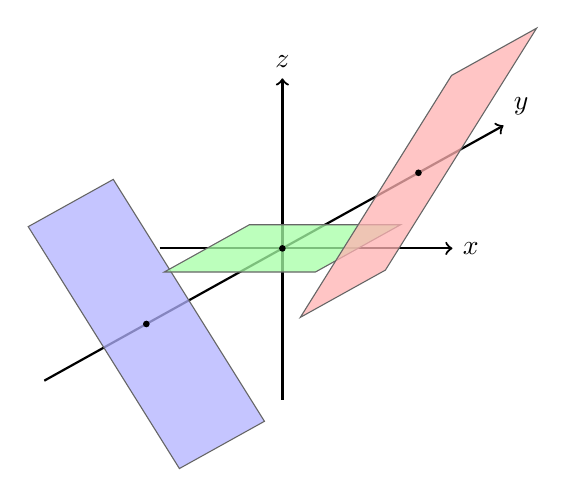
\begin{tikzpicture}[x={(1cm,0cm)},y={(0.9cm,0.5cm)},z={(0cm,1cm)},scale=1.2]
\draw[->,thick] (-1.3,0,0)--(1.8,0,0) node[right]{$x$};
\draw[->,thick] (0,-2.8,0)--(0,2.6,0) node[above right]{$y$};
\draw[->,thick] (0,0,-1.6)--(0,0,1.8) node[above]{$z$};
\foreach \yy/\col in {-1.6/blue!30,0/green!35,1.6/red!30}{
 \fill[\col,opacity=0.75] (-0.8,{\yy-0.5},{-0.8*\yy})--(0.8,{\yy-0.5},{0.8*\yy})--(0.8,{\yy+0.5},{0.8*\yy})--(-0.8,{\yy+0.5},{-0.8*\yy})--cycle;
 \draw[black!60] (-0.8,{\yy-0.5},{-0.8*\yy})--(0.8,{\yy-0.5},{0.8*\yy})--(0.8,{\yy+0.5},{0.8*\yy})--(-0.8,{\yy+0.5},{-0.8*\yy})--cycle;
 \fill (0,\yy,0) circle (1pt);
}
\end{tikzpicture}
\caption{接触平面 $\ker(\dd z-y\,\dd x)$。$y$ 軸に沿って平面は（$x$ 方向の傾き $\dd z/\dd x=y$ が変わりながら）ねじれていく。ねじれのため、どの平面も積分曲面に延びない。}\label{A:fig:contact}
\end{figure}

\begin{keybox}{§3 の要点}
\begin{itemize}
\item 接ベクトルの 3 つの定義（導分／曲線の速度／座標成分 $v'^j=\frac{\partial y^j}{\partial x^i}v^i$）は同値。$T_pM$ は $n$ 次元で、座標ベクトル $\partial_i$ が基底。
\item $\dd F_p$ は Jacobi 行列で、連鎖律 $\dd(G\circ F)=\dd G\circ\dd F$。$TM$、$T^*M$ は $2n$ 次元多様体。
\item ベクトル場の流れ（ODE）は最大流 $\theta:\mathcal D\to M$ で、コンパクト台ならば完備。
\item $[X,Y]f=X(Yf)-Y(Xf)$、成分 $X^i\partial_iY^k-Y^i\partial_iX^k$、Jacobi 恒等式と Leibniz 則。$[X,Y]=\Lie_XY=\frac{\dd}{\dd t}\phi_{-t*}Y$ で、$[X,Y]=0\Leftrightarrow$ 流れが可換 $\Leftrightarrow$ 座標ベクトル場。
\item Lie 群の左不変ベクトル場の括弧が Lie 代数。$\mathfrak{gl}(n)$ の括弧は交換子、$\mathfrak{so}(3)\cong(\R^3,\times)$。
\item \textbf{Frobenius}：分布は包合的であることと可積分（座標 $\partial_1,\dots,\partial_k$ の張る分布）であることが同値。非可積分の例が接触構造 $\ker(\dd z-y\,\dd x)$。
\end{itemize}
\end{keybox}

\subsection*{§3 のつまずきやすい点}
\begin{enumerate}
\item \textbf{成分は反変、座標ベクトルは共変。}$v'^j=\frac{\partial y^j}{\partial x^i}v^i$ と $\partial_{x^i}=\frac{\partial y^j}{\partial x^i}\partial_{y^j}$ では、行列が同じ $\frac{\partial y}{\partial x}$ で、$v=v^i\partial_{x^i}=v'^j\partial_{y^j}$ が整合する。
\item \textbf{座標ベクトル場 $\partial_{x^1}$ は他の座標 $x^2,\dots$ にも依存する。}$\partial_r$ は、座標 $(r,\theta)$ で決まるので、$\varphi=\theta+r$ として座標 $(r,\varphi)$ をとると別のベクトル場になる（$\partial_r|_{(r,\varphi)}=\partial_r|_{(r,\theta)}-\partial_\theta$）。座標ベクトル場は「座標系全体」で決まる。
\item \textbf{Lie 括弧は 2 階の項が消えるので 1 階の微分作用素。}成分式の符号を暗記するより、$[X,Y]f=X(Yf)-Y(Xf)$ に戻って計算するのが安全。
\item \textbf{左不変と右不変、基本ベクトル場の符号。}Lie 代数を左不変ベクトル場で定義すると $[A,B]=AB-BA$。作用が生成するベクトル場は反準同型になる。
\item \textbf{Frobenius は局所的。}可積分でも、葉は大域的には閉じていない（無理数 Kronecker 流の葉は稠密）。
\end{enumerate}

\subsection*{§3 の問題}
\begin{probl}{基本}{A_polar}
$\R^2\setminus\{0\}$ の極座標 $(r,\theta)$、$x=r\cos\theta$、$y=r\sin\theta$ について、(a) $\partial_r=\frac{x\partial_x+y\partial_y}{r}$、$\partial_\theta=x\partial_y-y\partial_x$ を連鎖律（\eqref{A:eq:coordvec}）から導け。(b) $\dd r$、$\dd\theta$ を $\dd x,\dd y$ で表し、$\dd\theta(\partial_\theta)=1$、$\dd r(\partial_\theta)=0$ を確かめよ。(c) $v=\partial_x$ の $(r,\theta)$ 成分を求めよ。
\end{probl}

\begin{probl}{基本}{A_bracket}
(a) $\R^2$ で $[R,E]=0$（$R=x\partial_y-y\partial_x$、$E=x\partial_x+y\partial_y$）。(b) $\R$ 上で $e_n=x^{n+1}\partial_x$ とおくと $[e_m,e_n]=(n-m)e_{m+n}$（Witt 代数）。(c) $\R^3$ 上で $[\partial_x+y\partial_z,\ \partial_y]$ と $[\,x\partial_x+y\partial_y+z\partial_z,\ \partial_x]$ を求めよ。
\end{probl}

\begin{probl}{標準}{A_jacobi}
(a) Jacobi 恒等式を、$[X,[Y,Z]]f$ を展開して直接示せ。(b) $[fX,gY]=fg[X,Y]+f(Xg)Y-g(Yf)X$ を示せ。(c) $X=x\partial_y$、$Y=y\partial_z$、$Z=z\partial_x$ について $[X,Y]$、$[Y,Z]$、$[Z,X]$ を求め、Jacobi 恒等式を成分式で確かめよ。
\end{probl}

\begin{probl}{基本}{A_flow}
次のベクトル場の流れを求め、完備か否かを判定せよ。(a) $\R$ 上の $X=-x\partial_x$。(b) $\R^2$ 上の $X=y\partial_x$。(c) $\R^2$ 上の $X=x\partial_x+y\partial_y$。(d) $(0,\infty)$ 上の $X=\partial_x$（$\R$ の開区間）。(e) $\R$ 上の $X=x^2\partial_x$ の流れの定義域 $\mathcal D$ を図示せよ。
\end{probl}

\begin{probl}{発展}{A_complete}
$X=X^i\partial_i$ を $\R^n$ 上の滑らかなベクトル場で、線形増大 $|X(x)|\le C(1+|x|)$ をみたすとする。$X$ が完備であることを示せ。\hint{積分曲線 $\gamma$ が $[0,\omega)$（$\omega<\infty$）で定義されるとして $u(t)=1+|\gamma(t)|$ に Grönwall を使い、$\gamma$ が有界であることを示し、脱出補題（定理~\ref{A:thm:ode}(4)）に矛盾させる。}
\end{probl}



\begin{probl}{基本}{A_loop}
(a) $X=x\partial_x$、$Y=\partial_x$ の流れ $\phi_t(x)=e^tx$、$\psi_t(x)=x+t$ について $\psi_{-t}\phi_{-t}\psi_t\phi_t(x)$ を計算し、$x-t^2+O(t^3)$ になること、これが $t^2[X,Y]=-t^2\partial_x$ と一致することを確かめよ。(b) $X=\partial_x$、$Y=\partial_y$ では閉じること、$[X,Y]=0$ との関係を述べよ。
\end{probl}

\begin{probl}{基本}{A_liealg}
(a) 例~\ref{A:ex:so3} の行列 $L_i$ について $[L_1,L_2]=L_3$、$[L_2,L_3]=L_1$、$[L_3,L_1]=L_2$ を計算で確かめよ。(b) $L_iv=e_i\times v$ を示し、$\omega\times$ に対応する行列 $\hat\omega$ について $[\hat\omega,\hat\eta]=\widehat{\omega\times\eta}$ を（ベクトル積の Jacobi 恒等式から）導け。(c) $\mathfrak{su}(2)=\{A\in M_2(\C):A^*=-A,\tr A=0\}$ で $e_k=-\frac i2\sigma_k$（$\sigma_k$ は Pauli 行列）について $[e_i,e_j]=\varepsilon_{ijk}e_k$。したがって $\mathfrak{su}(2)\cong\mathfrak{so}(3)$。(d) $\R^3$ 上の線形ベクトル場 $\hat L_1=y\partial_z-z\partial_y$ などについて $[\hat L_1,\hat L_2]=-\hat L_3$ を成分式で確かめ、符号の違いの理由を述べよ。
\end{probl}


\begin{probl}{標準}{A_frob}
(a) $\R^3$ で $D=\mathrm{span}(\partial_x+y\partial_z,\ \partial_y+x\partial_z)$ は包合的であることを示し、可積分座標（$D$ を張る $\partial_1,\partial_2$ となる座標）を求めよ。\hint{$f=z-xy$ の等位面} (b) $D'=\mathrm{span}(\partial_x+z\partial_y,\ \partial_z)$ は包合的でないことを示せ。(c) $\R^3\setminus\{0\}$ 上の $D''=\{v:p\cdot v=0\}$（$p$ は位置ベクトル、$D''=\ker(x\dd x+y\dd y+z\dd z)$）が包合的であることを示し、葉を求めよ。\hint{$R_1=y\partial_z-z\partial_y$、$R_2=z\partial_x-x\partial_z$、$R_3=x\partial_y-y\partial_x$ は $D''$ の切断。$z\ne0$ で $R_1,R_2$ が局所枠で、$[R_1,R_2]=-R_3=(xR_1+yR_2)/z$。}
\end{probl}

\begin{probl}{標準}{A_kron}
$T^2$ 上の $X=\partial_x+a\partial_y$（例~\ref{A:ex:kronecker}）について、閉曲線 $\{x=0\}$ への\emph{第一回帰写像}は $y\mapsto y+a\pmod1$ であることを示し、(a) $a=p/q$ なら各積分曲線は閉じ、(b) $a$ が無理数なら各積分曲線は $T^2$ で稠密であることを示せ。
\end{probl}

\begin{probl}{標準}{A_contact}
$\alpha=\dd z-y\,\dd x$、$D=\ker\alpha$。(a) $\alpha\wedge\dd\alpha=\dd z\wedge\dd x\wedge\dd y$ を計算せよ（$\dd\alpha=-\dd y\wedge\dd x$）。(b) $D$ の接線をもつ曲線（水平曲線）$\gamma(t)=(x(t),y(t),z(t))$ について $\dot z=y\dot x$ である。$(x,y)$ 平面の半径 $r$ の円周を反時計回りに 1 周する水平曲線の $z$ の増分が $-\pi r^2$ であることを示せ（Green の公式 $\oint y\,\dd x=-\mathrm{面積}$）。(c) したがって原点から $(0,0,h)$ へ水平曲線で行けることを示せ（Chow の定理の例）。
\end{probl}
